\documentclass[conference]{IEEEtran}
\IEEEoverridecommandlockouts
% The preceding line is only needed to identify funding in the first footnote. If that is unneeded, please comment it out.
\usepackage{cite}
\usepackage{amsmath,amssymb,amsfonts}
\usepackage{algorithmic}
\usepackage{graphicx}
\usepackage{subcaption}
\usepackage{textcomp}
\usepackage[table, xcdraw]{xcolor}
\usepackage{booktabs}
\usepackage{lettrine}
\def\BibTeX{{\rm B\kern-.05em{\sc i\kern-.025em b}\kern-.08em
    T\kern-.1667em\lower.7ex\hbox{E}\kern-.125emX}}
    
\makeatletter
\def\endthebibliography{%
  \def\@noitemerr{\@latex@warning{Empty `thebibliography' environment}}%
  \endlist
}
\makeatother

\graphicspath{{figures/}}
\newtheorem{definition}{Definition}
\begin{document}
\title{Multi-modal Multi-objective Optimization: Problem Analysis and Case Studies
}
\author{\IEEEauthorblockN{Yiming Peng, Hisao Ishibuchi, Ke Shang}
\IEEEauthorblockA{\textit{Department of Computer Science and Engineering, Southern University of Science and Technology (SUSTech)} \\
\textit{Shenzhen Key Laboratory of Computational Intelligence}\\
Shenzhen, China \\
11510035@mail.sustech.edu.cn, hisao@sustech.edu.cn, kshang@foxmail.com}
}

\maketitle

\begin{abstract}
In many real-world applications, multi-objective optimization problems can contains more than one Pareto sets. The optimization goal of multi-modal multi-objective optimization is to find all Pareto sets in decision space. As a relatively new research area, the difficulties to solve multi-modal multi-objective optimization problem has not been carefully analyzed. In this article, we point out that traditional environmental selection, mutation and crossover mechanisms may cause problems when solving multi-modal multi-objective optimization problems. Furthermore, we creatively introduce the concept of genetic drift to explain the reduction of diversity in decision space during the evolution process. In addiction, this article also provide a comparative studies of state-of-the-art algorithms using a series of computational experiments.
\end{abstract}

\begin{IEEEkeywords}
Multi-modal multi-objective optimization, Genetic Drift, Evolutionary algorithms
\end{IEEEkeywords}

\section{Introduction}
\lettrine[lines=2]{M}{any} real-world optimization problems require to optimize more than one objective functions which are usually conflicting to each other. In most circumstances, the fitness improvement in one objective function will cause fitness deterioration in other objectives. We generally denote this kind of problems as Multi-objective Optimization Problems(MOPs). Multi-objective Evolutionary Algorithms(MOEAs) are designed for solving MOPs. Mainstream MOEAs usually follow "posterior" approach which assumes that no user preference information are provided before and during the optimization process. Therefore, MOEAs need to obtain a set of non-dominated solutions that is uniformly cover the Pareto Front(PF). Then the decision maker can select a subset from the obtained solutions according to user's preferences. As mentioned above, usually MOEAs only consider the diversity of solution set in objective space. Diversity in the decision space does not gain much attention. However, sometimes the diversity in decision space is also very important, especially for multi-modal multi-objective optimization problem(MMOP). MMOPs is a special kind of MOPs which contains more than one Pareto optimal solution sets(PS) corresponding to the same PF. There are many MMOPs in real-world applications such as multi-objective knapsack problems \cite{Jaszkiewicz2002}, game map generation problem \cite{Togelius} etc. An MMOP requires optimizer to obtain a solution set that cover as much Pareto sets as possible. In many engineering problems, some solutions are hard to implement due to physical limitations. In this case, obtaining multiple Pareto sets can help decision maker to select alternative solutions with equivalent quality in objective space. In addition, the knowledge about multiple Pareto optimal solution sets may be for better understanding of the structure of the optimization problem\cite{Deb2001}.

As pointed out in many literature\cite{Tanabe2019} \cite{Liang2016}, the performance of MOEAs on MMOPs are not good. Usually MOEAs only obtain single Pareto set. In this paper, we further confirm this proposition with a series of computational experiments. In addiction, in this article we have tried to make some analysis and explanations on why MOEAs perform poor on MMOPs. We reveal that in order to find solutions in all Pareto sets, an explicit mechanism to maintain the solution diversity in decision space is necessary. This means that the algorithm should be able to maintain the diversity of the solutions in both decision and objective space. For convenience, evolutionary algorithms designed for solving MMOPs are known as Multi-modal Multi-objective Evolutionary Algorithms or MMEAs in short. Since 2005, MMEAs has begun to receive attention from community researchers. Some new algorithms are specially designed for MMOPs and some of them are modified from existing MOEAs. But currently there is no comparison of the performance between them. In this paper, several popular MMEAs are tested and their performance on the test problems with different dimensional decision space are studied. We also examine the effectiveness of MMEAs on solving MMOPs compared to classical MOEAs.

The structure of this paper is as follows. In section \ref{Multi-modal Multi-objective Optimization}, we give the formal definition of MMOPs. Section \ref{Difficulties Analysis} reveals the difficulties of solving MMOPs. In section \ref{Review of State-of-the-art Techniques}, mainstream diversity maintenance techniques in the literature and their characteristics are reviewed. Section \ref{Experimental Settings} is devoted to describe the experimental settings. Then a series of computational experiments are conducted in section \ref{Experimental Results}. Finally, we conclude this paper.
\section{Multi-modal Multi-objective Optimization}
\label{Multi-modal Multi-objective Optimization}
\subsection{Formal Definition}
The formal definition of MMOPs can be described as follows\cite{Tanabe2019}:
\begin{definition}
An MMOP is a kind of MOP that requires to find all solutions that are equivalent to Pareto optimal solutions. 
\end{definition}
\begin{definition}
Solutions $\boldsymbol{x_1}$ and  $\boldsymbol{x_2}$ are equivalent  iff $||f(\boldsymbol{x_1}) - f(\boldsymbol{x_1})|| \leq \delta$ .
\end{definition}

Where $\delta$ is a positive number that represents the tolerance of similarity of solutions given by the decision maker. If $\delta = 0$, decision maker only accept Pareto optimal solutions and the dominated solutions should be removed in the final population.  Larger $\delta$ means that decision maker can accept the sub-optimal solutions that are more inferior than Pareto optimal solutions. Because it is difficult to accurately describe the relationship between the value of $\delta$ and the quality of the resulting solutions, in order to simplify the process of analysis, we only consider the case of $\delta =0$. 

\subsection{Multi-Polygon Test Problem}
There are several benchmark MMOPs used in existing literature such as Two-On-One \cite{Preuss2006}, Omni-test \cite{Deb2005} , SYM-PART \cite{Rudolph2007a} and Multi-Polygon test problem proposed in \cite{Hisao} etc. This paper use Multi-Polygon test problem for analyzing the performance of MOEAs and MMEAs because it has better flexibility than other test problems.  Multi-Polygon test problem is a MMOPs based on the idea of distance minimization. For example, there are four identical regular hexagons with radius $r$ in figure \ref{fig:Multi-Polygon Problem}, and the distance $l$ between any two adjacent polygons are larger than $4r$ (Please refer to \cite{Hisao} for more details about the specification of $l$). With these settings, we can define a 6-objective optimization problem by:

\begin{equation*}
\left\{
\begin{array}{c}{f_{1}(\boldsymbol{x})=\min \left\{d\left(\boldsymbol{x}, A_{1}\right), d\left(\boldsymbol{x}, B_{1}\right), d\left(\boldsymbol{x}, C_{1}\right), d\left(\boldsymbol{x}, D_{1}\right)\right\}} \\ \dots \\ {{f_{6}}(\boldsymbol{x})=\min \left\{d\left(\boldsymbol{x}, A_{6}\right), d\left(\boldsymbol{x}, B_{6}\right), d\left(\boldsymbol{x}, C_{6}\right), d\left(\boldsymbol{x}, D_{6}\right)\right\}}\end{array}
\right.
\end{equation*}

Where $d(\boldsymbol{a} ,\boldsymbol{b})$ is the Euclidean distance between vector $\boldsymbol{a}$ and $\boldsymbol{b}$.  In this test problem, any point inside the four hexagons is Pareto optimal solutions. Therefore, this test problem has four equivalent Pareto sets. One of the biggest advantage of this test problem is that the dimension of its decision space can be extended by mapping the plane to a two-dimensional subspace in any dimension space. 

\begin{figure}[htbp]
	\centering
	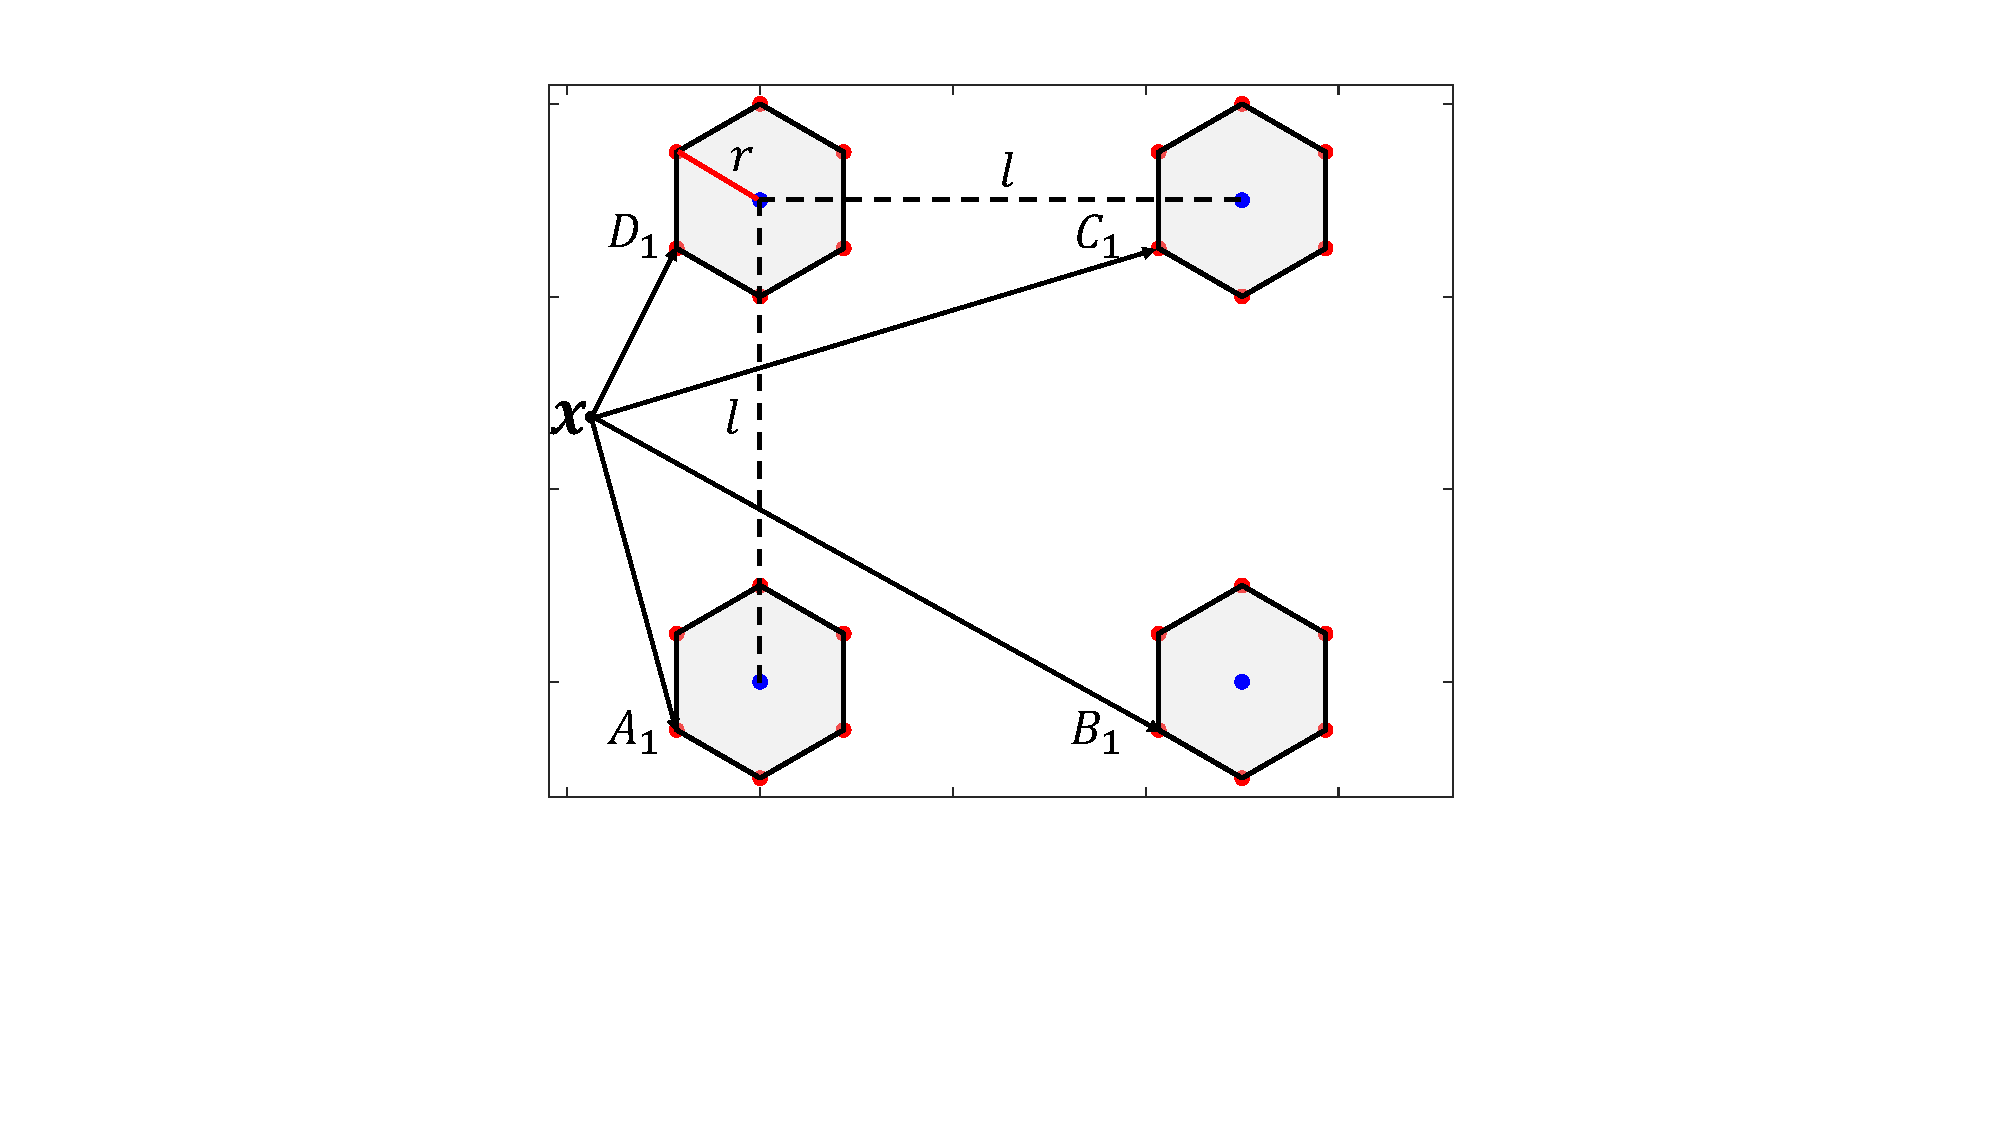
\includegraphics[width=.3\textwidth]{Section2/Problem}
	\caption{An example of Multi-Polygon test problem.}
	\label{fig:Multi-Polygon Problem}
\end{figure}

\section{Difficulties Analysis}
\label{Difficulties Analysis}
Although there have been a lot of researches on MMOPs, the analysis of the difficulty of solving the MMOPs is still relatively rare. In this section, we analyzed the difficulty of  maintaining the diversity of populations in the decision space. Because at different stages of evolution, the reasons for affecting the distribution of population in the decision space may varies. We can use the IGD value to divide the evolutionary process into different phases.

Suppose that IGD values of the population at $t$ evaluations and final population are $V_t$ and $V_f$ respectively. We define a relative error function $\delta_e(t)$ as :
$$\delta_e(t)=\frac{|V_t-V_f|}{V_f}$$
Then we can say that the population become mature at $T$ evaluations iff $\forall t<T$, $\delta_e(t)>\Delta$ and $t \ge T$, $\delta(t) \leq \Delta$. Where $\Delta$ is threshold define by user. As shown in figure \ref{fig: Two stages}, the evolution process is separated into young and mature stage using $\Delta=3\%$.
\begin{figure}[htbp]
    \centering
    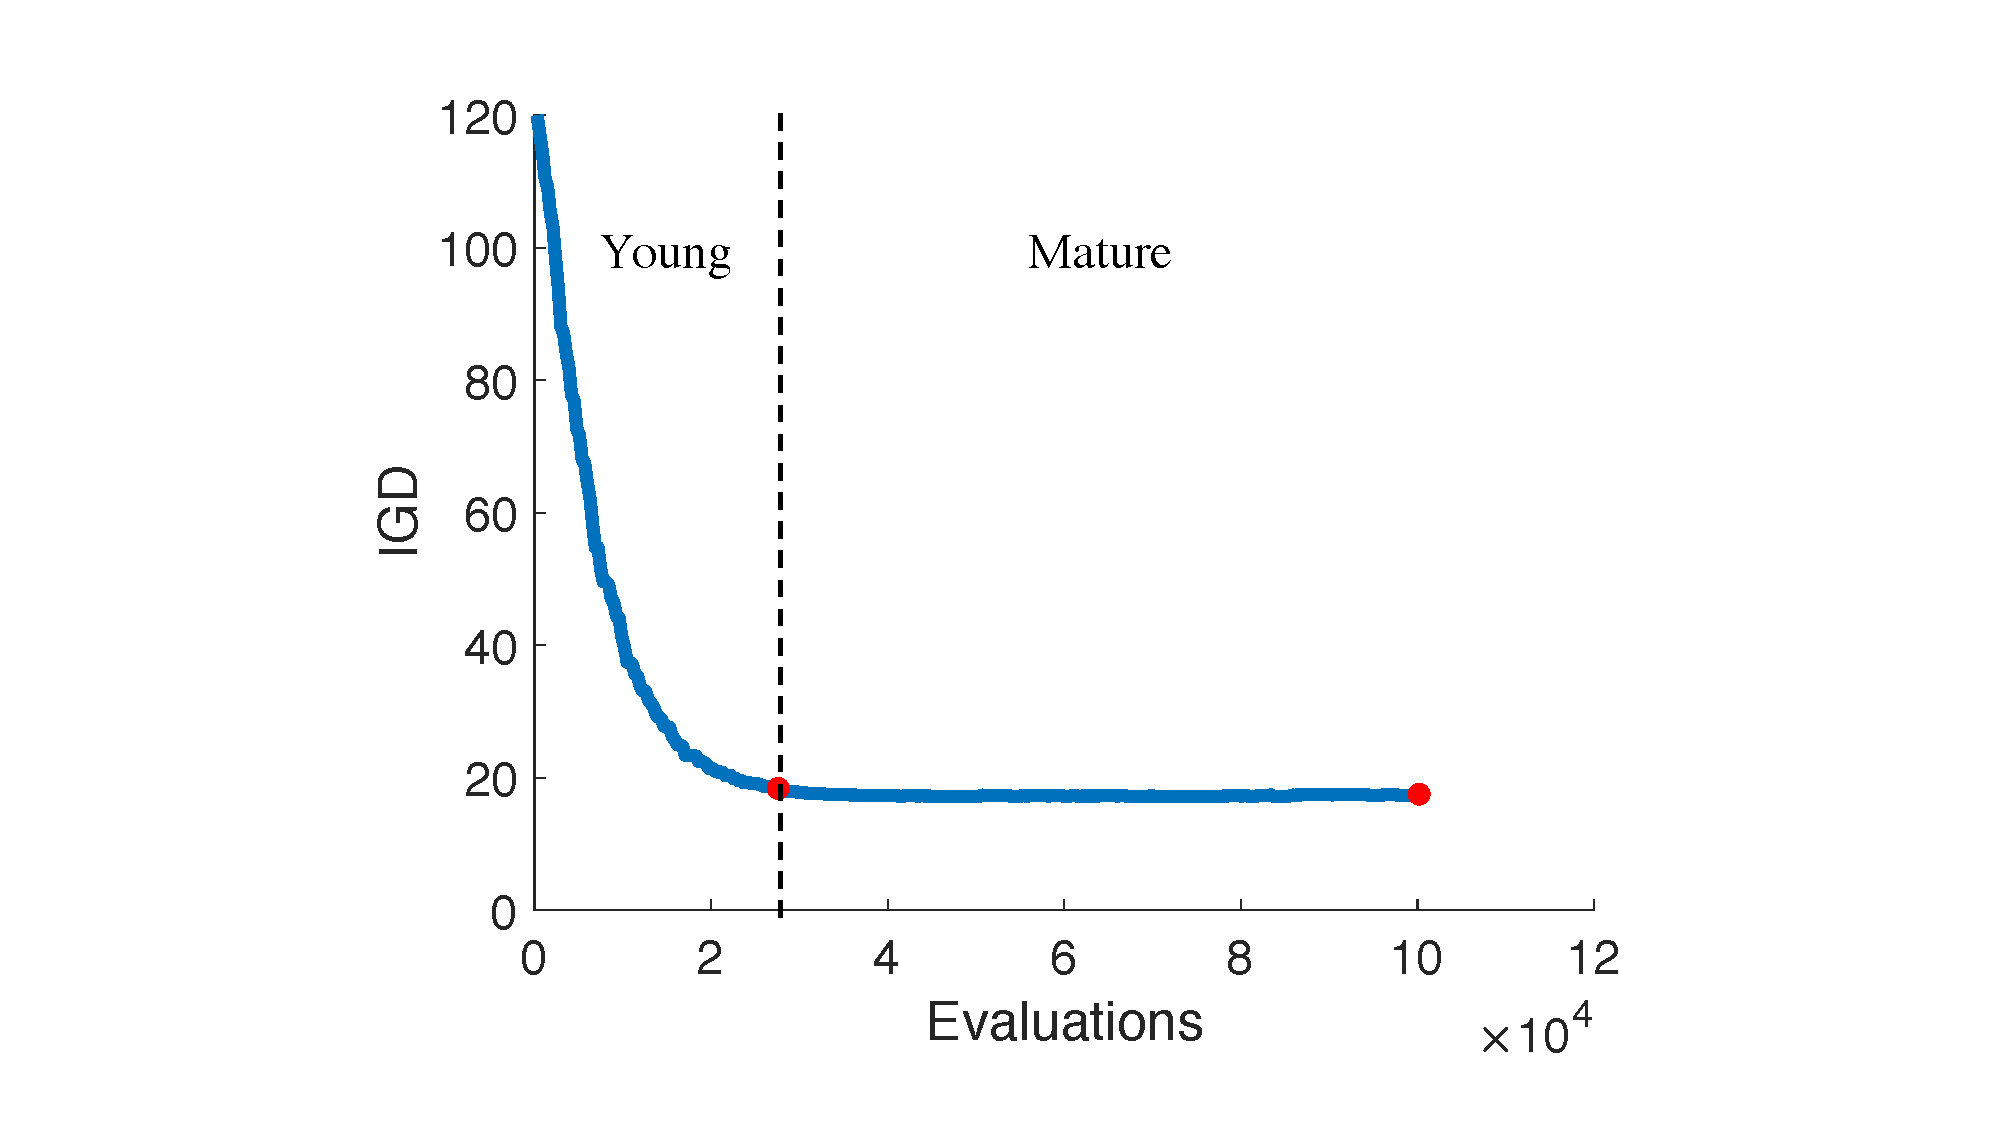
\includegraphics[width=.35\textwidth]{Section3/Stages}
    \caption{Two stages of evolution process.}
    \label{fig: Two stages}
\end{figure}

In the young stage, the individuals in the population are far away from the PF. And in the mature stage, the whole population is very close to PF but the distribution of population in decision space may change. Now we address the difficulties for solving MMOPs from the following three aspects:

\subsection{Environmental Selection}
\label{Impact of environmental selection}
For most MOEAs, the environmental selection acts on whole population. This will cause two consequences:
On one hand, in the young stage of the evolution, a relatively good solution will quickly lead to other potential solutions which is far away from it in decision space to extinction. 
On the other hand, as pointed out in \cite{Liang2016}, for MMOPs, two solutions that are very far apart in the decision space may be very close in the objective space. Then MOEAs will remove the solutions that are too crowded in the objective space, therefore equivalent(or slightly inferior) solutions will be eliminated in mature stage. As figure \ref{fig: Environmental selection} shows, for both cases, the diversity of the population in decision space will decrease. 

\begin{figure}[htbp]
	\centering
	\begin{subfigure}[b]{.3\textwidth}
		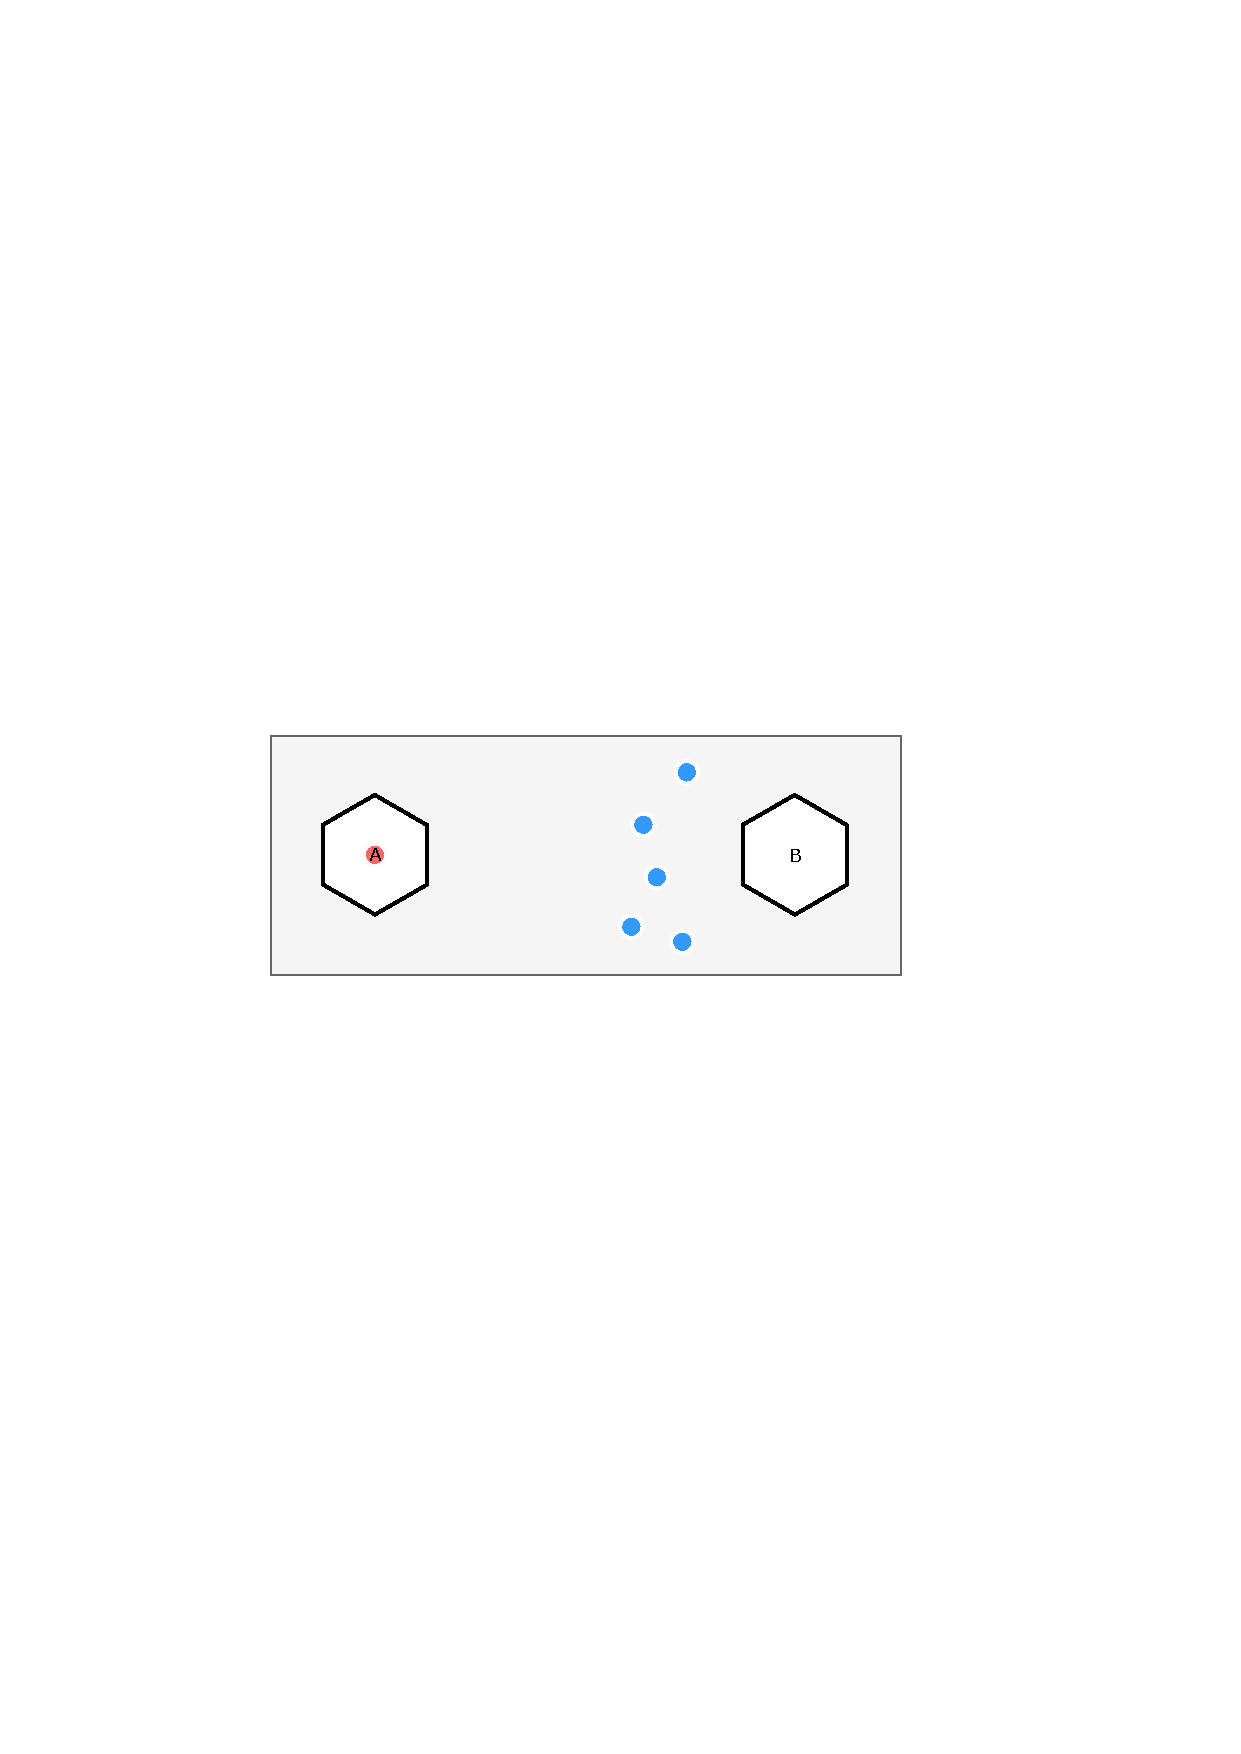
\includegraphics[width=\linewidth]{Section3/case1}
		\caption{Case 1}
	\end{subfigure}
	\begin{subfigure}[b]{.3\textwidth}
		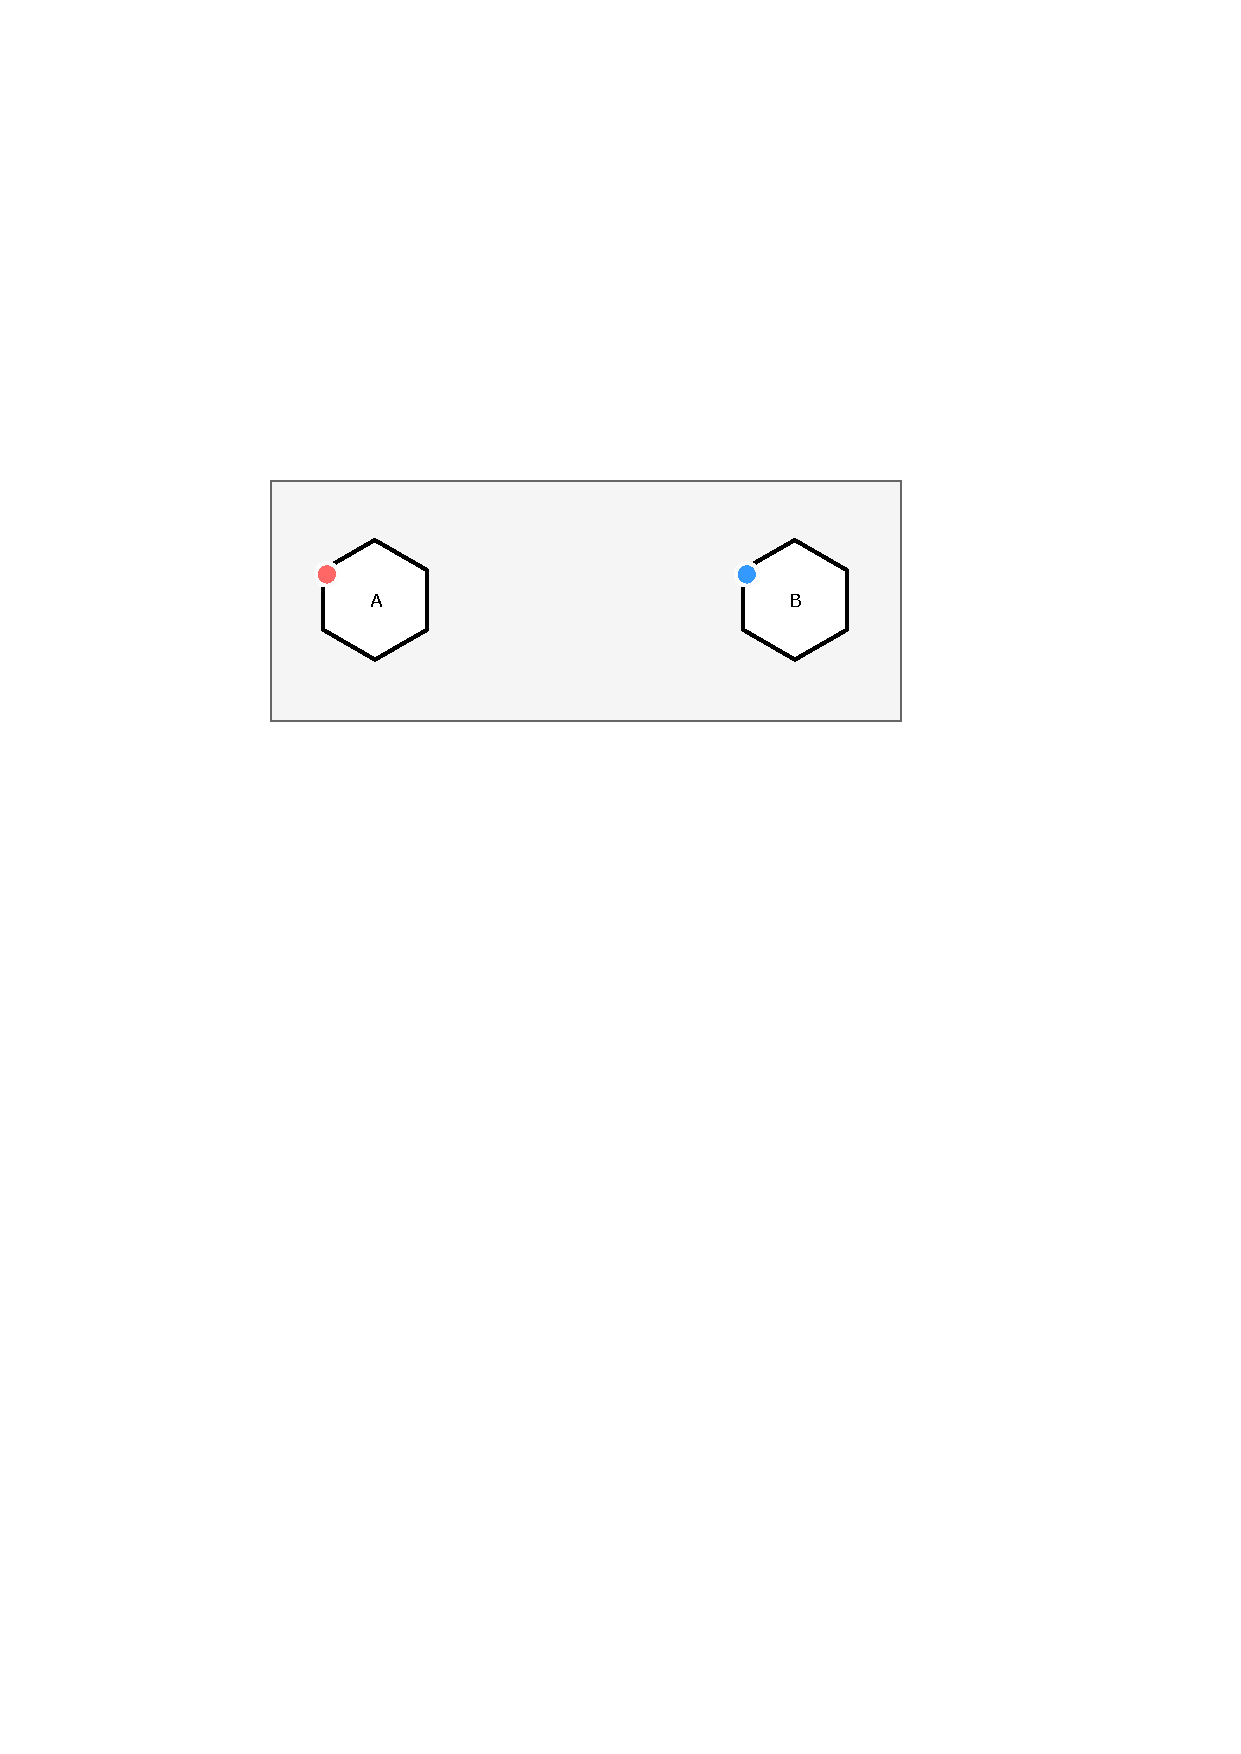
\includegraphics[width=\linewidth]{Section3/case2}
		\caption{Case 2}
	\end{subfigure}
	\caption{The impact of environmental selection on the diversity of population in the decision space. In each case, only the red circle survive in next generation.}
	\label{fig: Environmental selection}
\end{figure}


\subsection{Genetic Drift}
The reduction of the diversity in decision space also related to a phenomena called Genetic Drift. Genetic drift is a phenomena in which the frequency of alleles in a population declines due to random sampling errors \cite{GeneticDrift}. Figure  \ref{fig:Genetic drift demo} gives an example of genetic drift. At generation $t$, the population contains same number of alleles $A$ and $a$, and we assume that only random sampling without selection, mutation and crossover from generation $t$ to $t+1$. Then due to the random sampling error, the frequency of $A$ becomes larger than $a$ in generation $t+1$. 

\begin{figure}[htbp]
	\centering
	\begin{subfigure}[b]{.3\textwidth}
		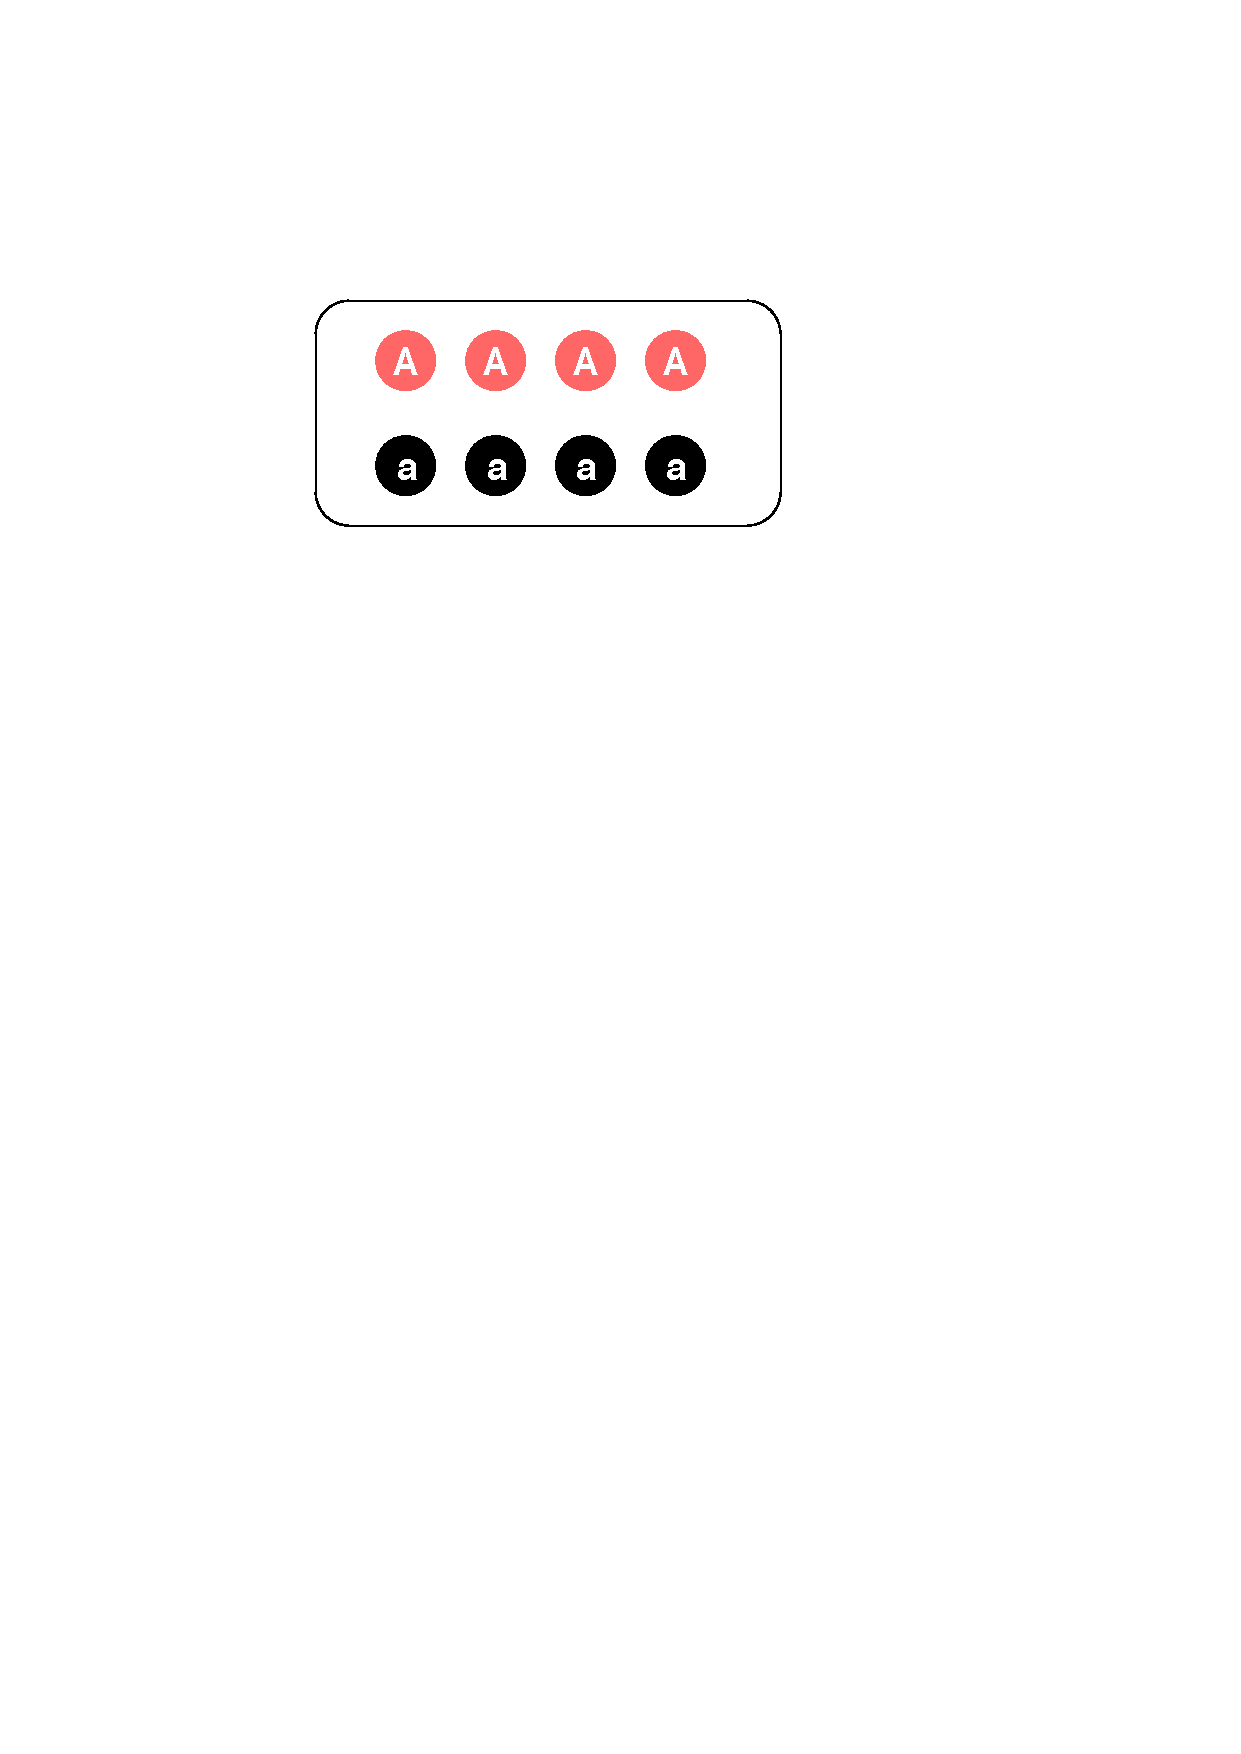
\includegraphics[width=\linewidth]{Section2/Generation_t}
		\caption{At time $t$, the population contains same number of alleles $A$ and $a$.}
	\end{subfigure}
	
	\begin{subfigure}[b]{.3\textwidth}
		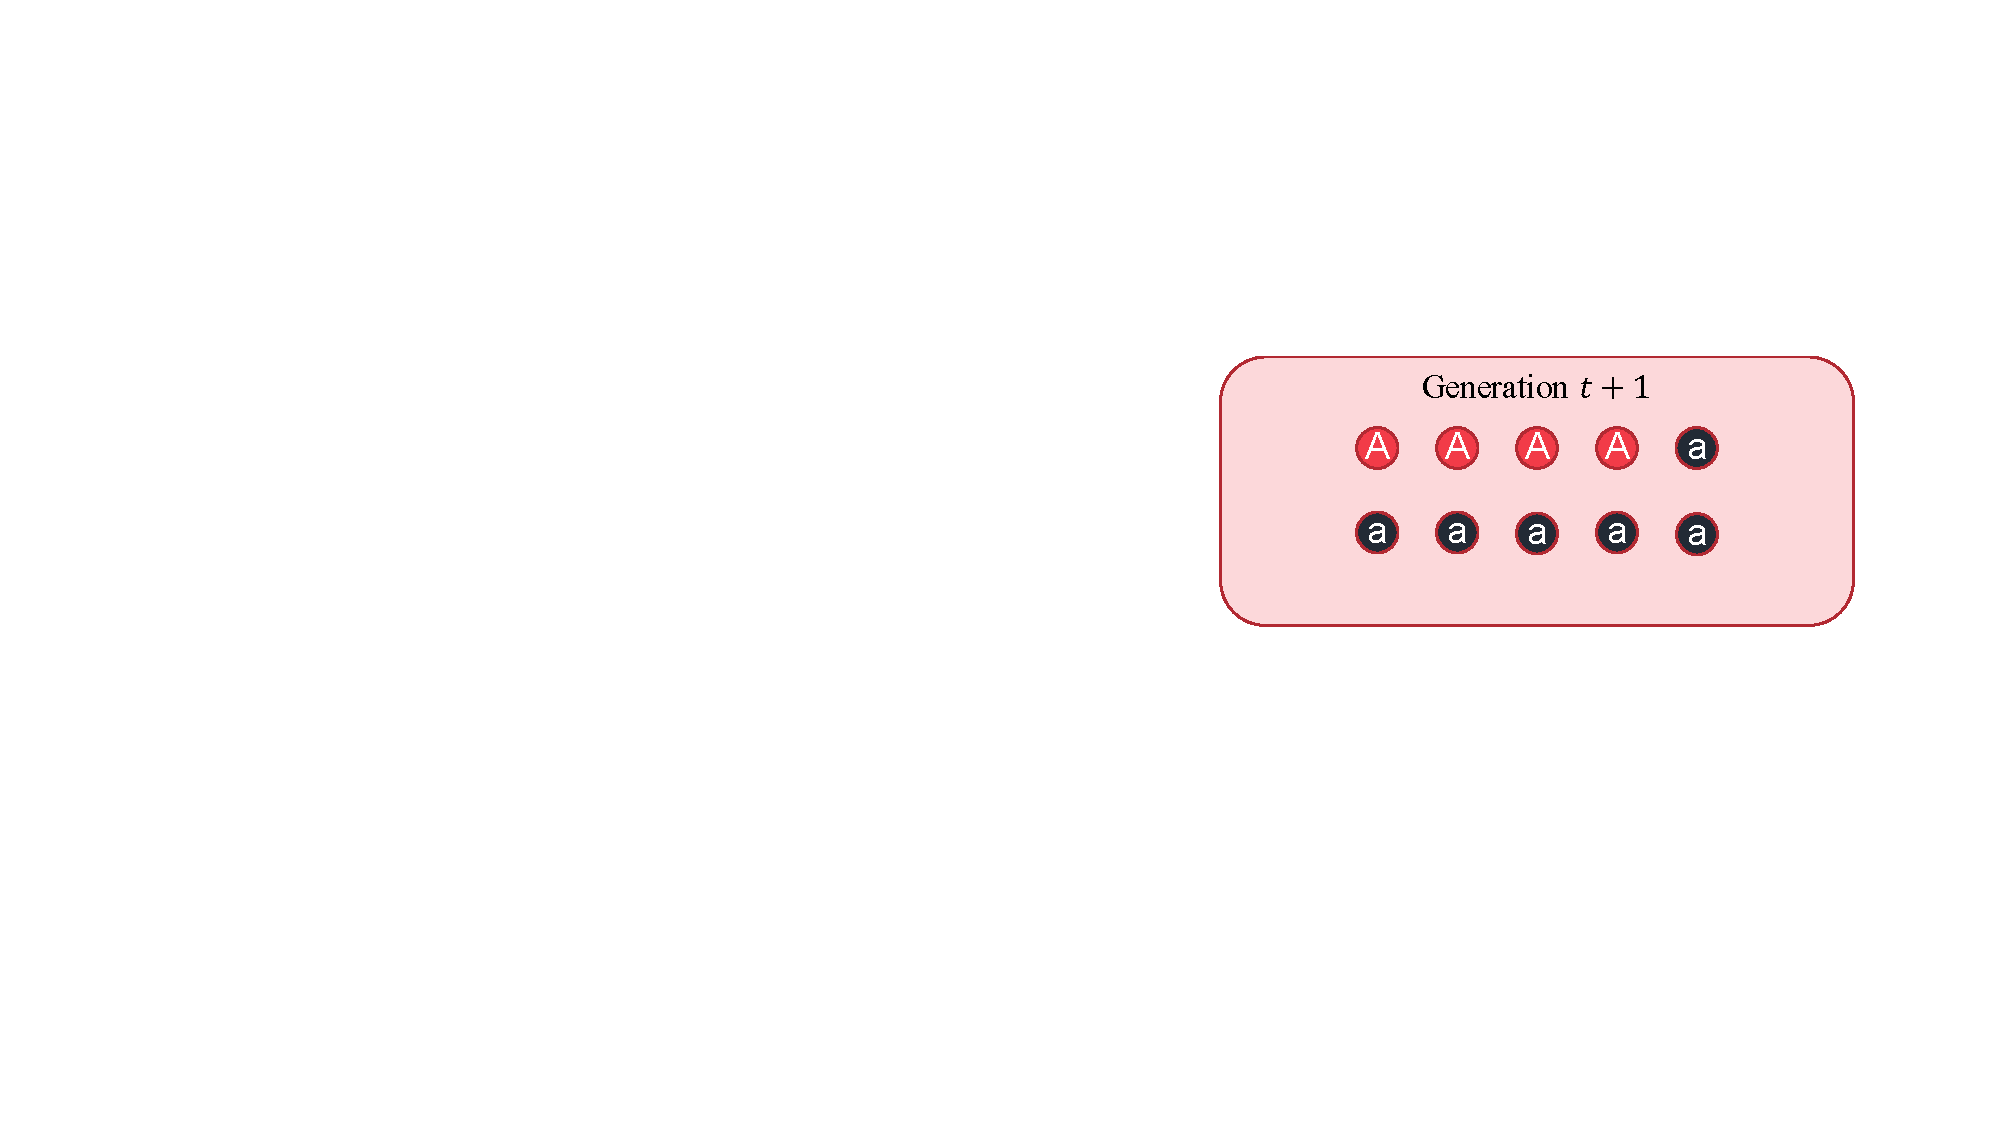
\includegraphics[width=\linewidth]{Section2/Generation_t1}
		\caption{At time $t+1$, due to random sampling error, $frequency(A) < frequency(a)$}
	\end{subfigure}
	\caption{Demonstration of genetic drift}
	\label{fig:Genetic drift demo}
\end{figure}

Genetic drift tend to reduce genetic variation of the population during the evolutionary process. Some of the alleles may even disappear due to genetic drift. Asoh\cite{Asoh} mathematically proved that with only random selection, as the iteration proceeds, only one of alleles in the population will survive(this process is called population convergence). And the mean convergence time is proportional to the population size. 

As shown in figure \ref{fig: Alleles}, when solving MMOPs, equivalent solutions can be seen as alleles because they are indistinguishable in terms of objective function values. Genetic drift can affect the distribution of population in the decision space throughout the evolution process. In general, due to the existence of genetic drift, all equivalent solutions in the population will be removed after a long enough evolution time. In section IV, we used more computational experiments to study the effects of genetic drift on solving MMOPs.

\begin{figure}[htbp]
    \centering
    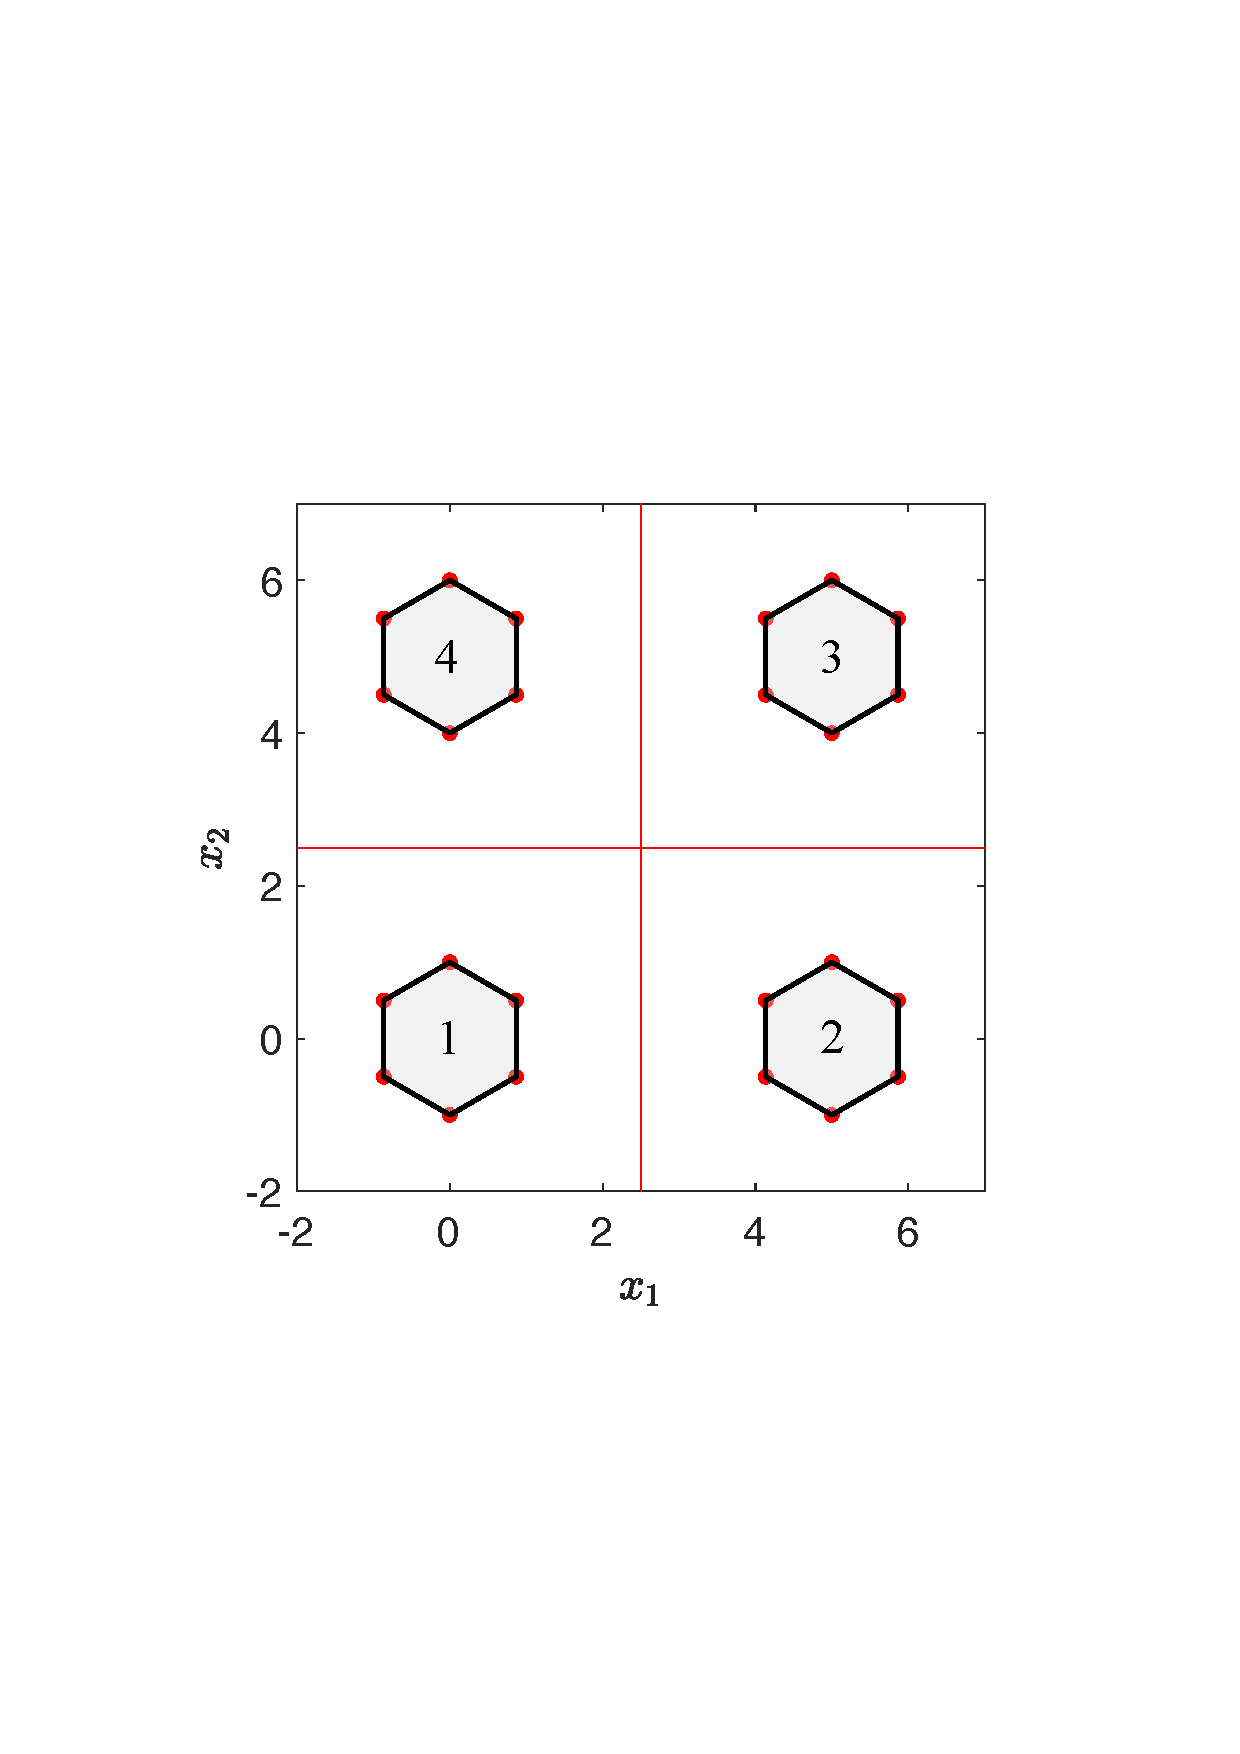
\includegraphics[width=.3\textwidth]{Section3/Alleles}
    \caption{Divide the decision space of Multi-Polygon test problem into 4 parts in counterclockwise order. Each part can be view as an gene allele.}
    \label{fig: Alleles}
\end{figure}

\subsection{Crossover and Mutation}
In evolutionary algorithms, crossover and mutation are two operation that will increase the variety of the population. These two techniques can help the algorithms to avoid trapping in the local optima. However, since mutation and crossover have higher probability of producing individuals that are close to their parents, the distribution of the parent population will affects the distribution of the offspring population. More specifically, more offspring will be produced in the region where the parent population has higher density. Figure \ref{fig: SBX crossover} demonstrates the results of generating 1,000 individuals from SBX\cite{SBX} with distribution index = 20. As shown in figure \ref{fig: SBX crossover case 1}, the diversity of solutions in decision space no change too much since now new alleles are generated. In figure \ref{fig: SBX crossover case 2}, the parents is set to two solutions in two diagonal polygons, i.e. $(0, 0)^T$ and $(5, 5)^T$. In this case, the diversity of solutions in decision space increase hugely, the number of alleles in the population increases from two to four. Figure \ref{fig: Polynomial mutation} depicts the results of polynomial mutation with distribution index = 20. Diversity in decision space not change too much. 

From these two simulation results, we can see that in the most cases, new alleles are hard to produced by crossover and mutation process. In the long run, crossover and mutation cannot provide enough variety to counter the effect of genetic drift. 
\begin{figure}[htbp]
	\centering
	\begin{subfigure}[b]{.24\textwidth}
		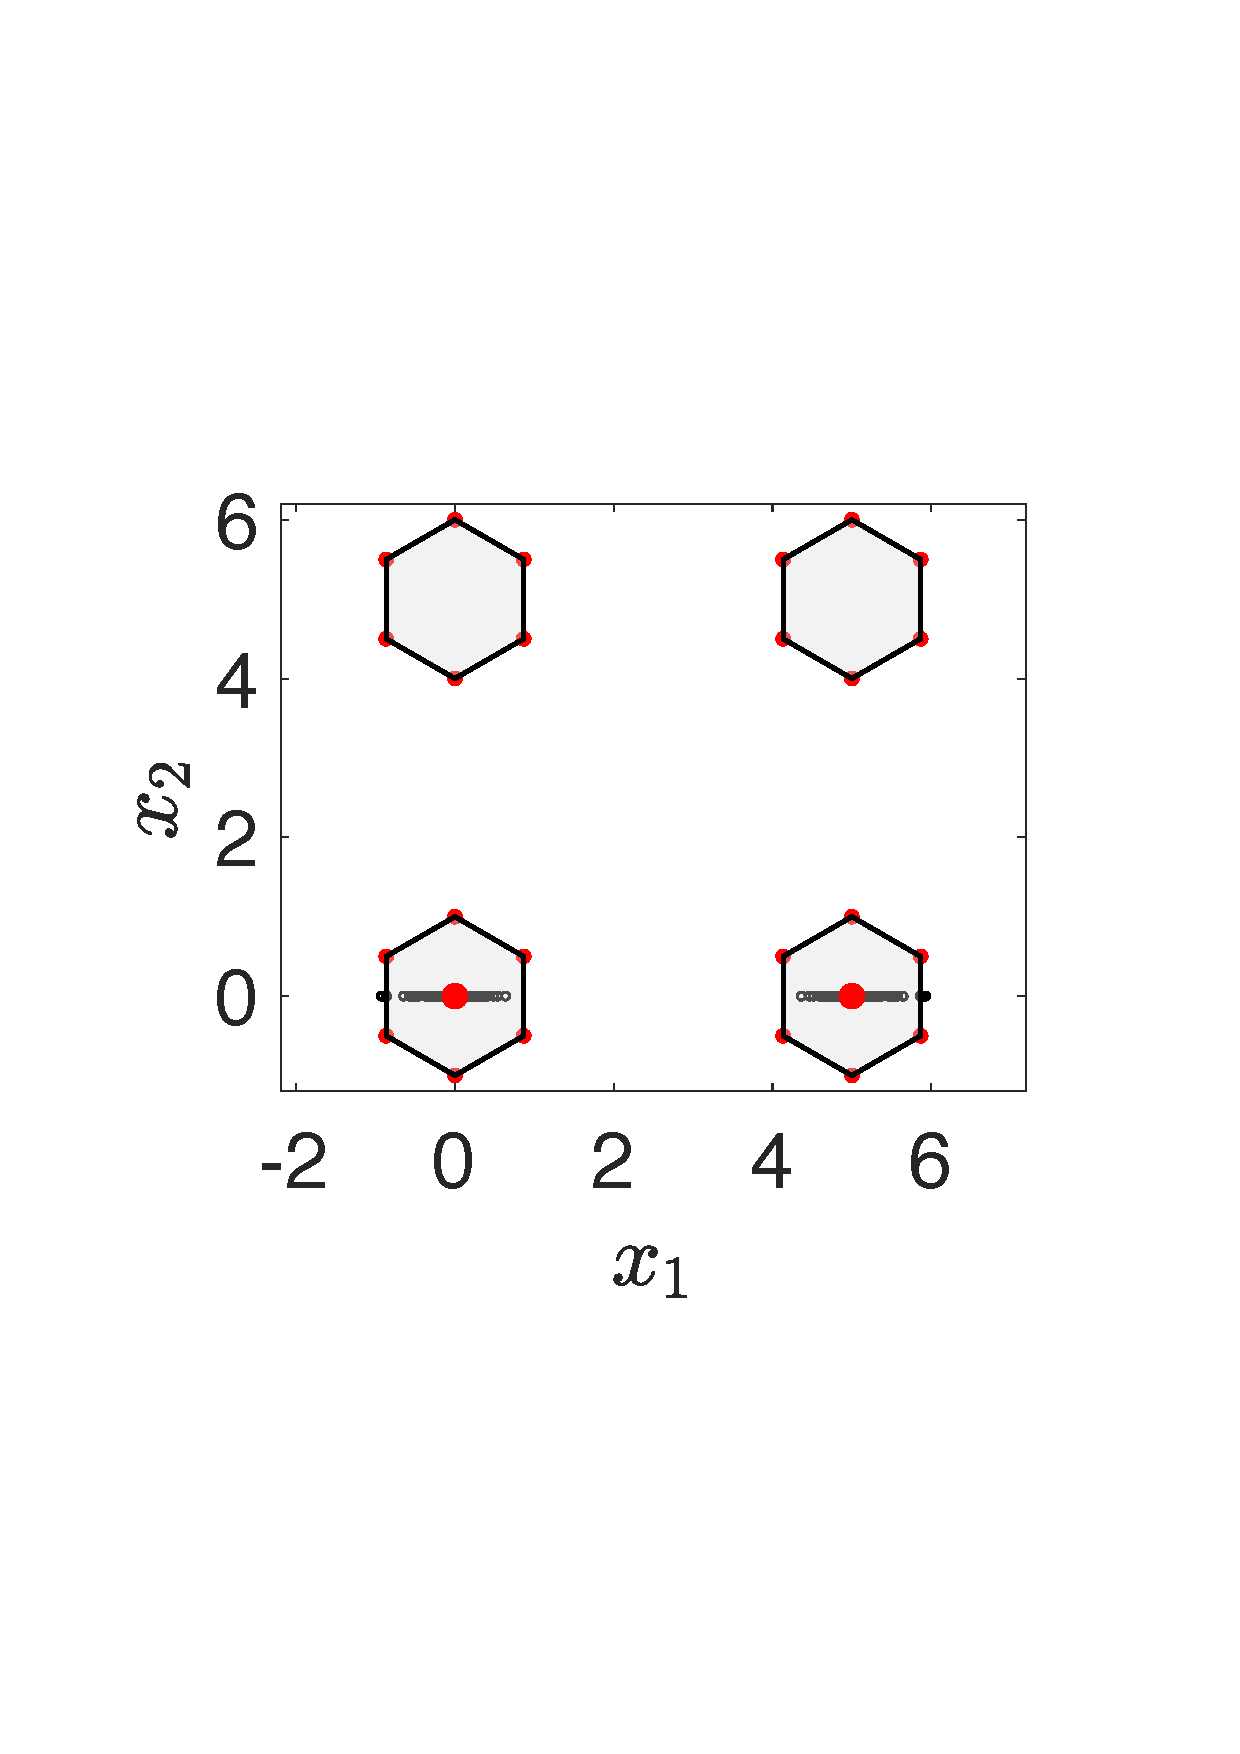
\includegraphics[width=\linewidth]{Section3/crossover1}
		\caption{Case 1: parents are $(0, 0)^T$ and $(5, 0)^T$. The number of alleles remains unchanged.}
		\label{fig: SBX crossover case 1}
	\end{subfigure}
	\begin{subfigure}[b]{.24\textwidth}
		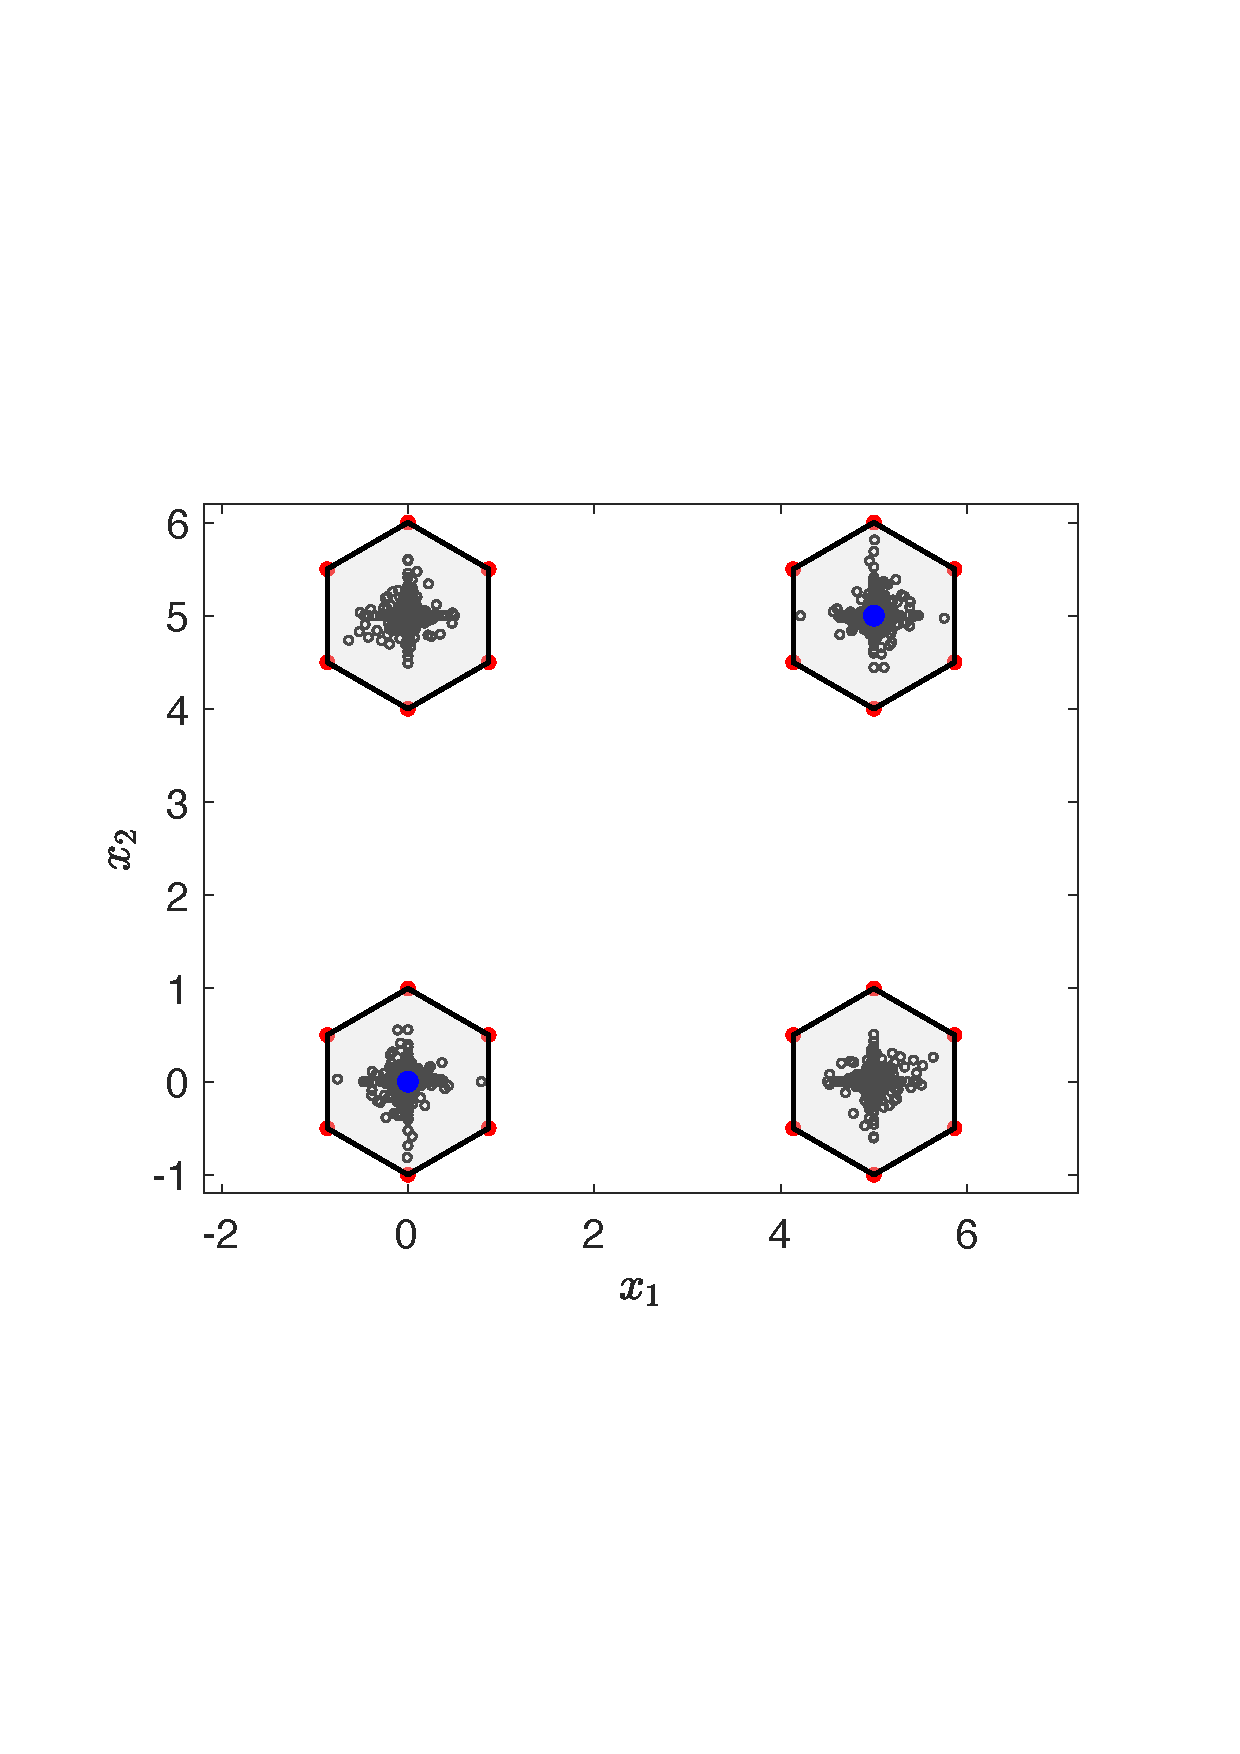
\includegraphics[width=\linewidth]{Section3/crossover2}
		\caption{Case 2: parents are $(0, 0)^T$ and $(5, 5)^T$. The number of alleles changes from 2 to 4.}
		\label{fig: SBX crossover case 2}
	\end{subfigure}
	\caption{Generate 1,000 individuals by SBX crossover. Blue and dark circles represent parent and offspring respectively.}
	\label{fig: SBX crossover}
\end{figure}

\begin{figure}[htbp]
    \centering
    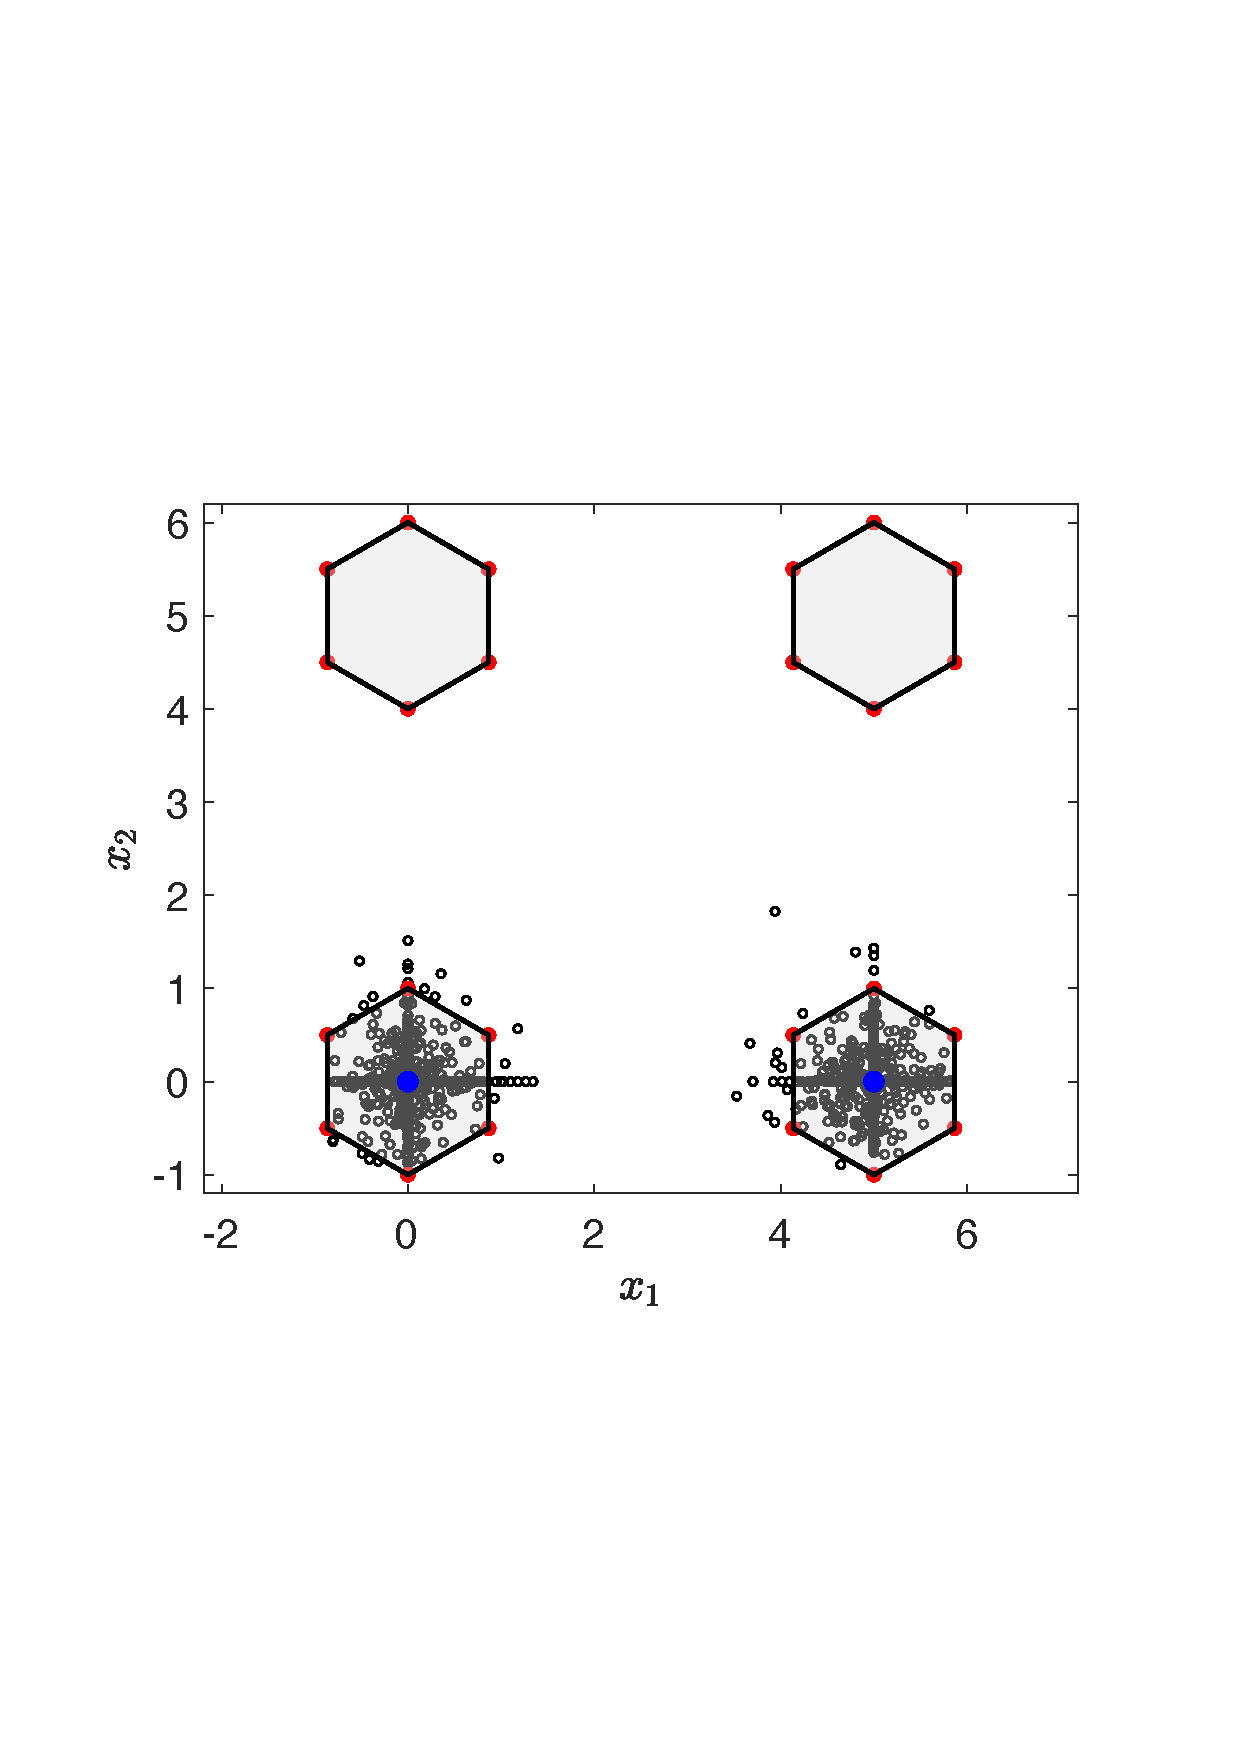
\includegraphics[width=.3\textwidth]{Section3/mutation}
    \caption{Generate 1,000 individual(shown in black) by applying polynomial mutation to two solutions(shown in blue). The number of alleles remains unchanged.}
    \label{fig: Polynomial mutation}
\end{figure}
\section{Review of State-of-the-art Techniques}
\label{Review of State-of-the-art Techniques}
In this section, we provide a short review of state-of-the-art techniques for maintain the diversity in the decision space. As pointed out by Deb \cite{Deb2001}, the key idea for solving MMOPs is to "divide" the entire population into several sub-population that do not affect each other as much as possible, and then let each sub-population evolve independently. Here we list some commonly used approaches:
\subsection{Fitness Sharing Approach}
Fitness sharing was first introduced in \cite{Goldberg} and widely adopted in MOEAs to keep the sparsity of the solutions in objective space. The key idea is to degrade the fitness of crowded solutions by sharing their fitness to neighborhood solutions. In order to solve MMOPs, fitness sharing in both decision and objective space need to be considered simultaneously. DNEA\cite{DNEA} used two fitness sharing function both in decision space and objective space. Fitness sharing approach is hard to apply because the sharing radius is problem dependent. In addition, combining fitness sharing in two spacing is also a challenging task.
\subsection{Crowding Distance Approach}
Crowding distance often used as a second selection criteria in Pareto-dominance based algorithms such as NSGA-II\cite{NSGA-II}. Several MMEAs such as Omni-optimizer\cite{Omni-Optimizer} and MO\_Ring\_PSO\_SCD\cite{MO-Ring-PSO-SCD} design special types of crowding distance that take both the decision and objective space into account.
\subsection{Restrict Environmental Selection Approach}
As discussed in section \ref{Impact of environmental selection}, carrying the environmental selection in whole population is harmful to the population diversity in decision space. Therefore one remedy is to restrict the environmental selection in part of solutions. More specifically, a solution should only compete with its neighborhood solutions in decision space. The neighborhood relationship may either distance based or index based. For example, in MOEA/D-AD \cite{MOEA/D-AD}, a solution $\boldsymbol{x}$ is only compete with the closest $L$ solutions in decision space by scalarizing function.

\section{Experimental Settings}
\label{Experimental Settings}
\subsection{Algorithms Selection}
In order to obtain more reliable experimental data, we have selected several representative MOEAs from the following three classes:
\begin{itemize}
    \item \textbf{Pareto-dominance based}: NSGA-II\cite{NSGA-II} and NSGA-III\cite{NSGA-III}.
    \item \textbf{Decomposition based}: MOEA/D \cite{MOEA/D} with PBI($\theta=20$) and Tchebycheff aggregation function.
    \item \textbf{Indicator based}: IBEA\cite{IBEA} and SPEA2\cite{SPEA2}.
\end{itemize}

Also, for MMEAs, we selected algorithms mentioned in section \ref{Review of State-of-the-art Techniques}: DNEA, MO\_Ring\_PSO\_SCD, MOEA/D-AD and Omni-Optimizer.
\subsection{Parameter Settings}
In these experiments, we used the following parameter settings: 
\subsubsection{GA Settings}
\begin{itemize}
    \item Population size $N$ = 300.
    \item Number of evaluations = 1e5.
    \item SBX crossover(distribution index = 20) with probability 1.0.
    \item Polynomial mutation(distribution index = 20) with probability $1/D$.
\end{itemize}
\subsubsection{Problem Settings}
\begin{itemize}
     \item Number of objectives $M=6$.
    \item Number of decision variables $D=2, 4$.
    \item Four regular polygons with radius $r=1$ and theirs centers are $\boldsymbol{c}_1=(0, 0)^T$, $\boldsymbol{c}_2=(5, 0)^T$, $\boldsymbol{c}_3=(5, 5)^T$, $\boldsymbol{c}_4=(0, 5)^T$. 
\end{itemize}
\subsubsection{Algorithm Settings}
We use default parameters for each algorithm according to corresponding article.
\begin{itemize}
    \item IBEA: fitness scaling factor $\kappa=0.05$.
    \item DNEA: niche radius in objective space $\theta_{obj}=0.06$ and niche radius in decision space $\theta_{var}=0.02$.
    \item MO\_Ring\_PSO\_SCD: the size of personal best archive $n_{PBA}=5$ and the size of neighborhood best archive $n_{NBA}=15$.
    \item MOEA/D-AD: use PBI($\theta=5$) aggregation function and neighborhood size $L = 0.1\mu$ where $\mu$ is the size of current population.
    \item Omni-optimizer: $\epsilon$-dominance parameter $\delta=0.001$.
\end{itemize}

\section{Experimental Results}
\label{Experimental Results}
In this section, we test the performance of selected MOEAs and MMEAs on Multi-Polygon test problem with different dimensional decision space. In each experiment, will run each algorithm 31 times and the run with median HV among them is reported. In addition, following similar manner from article \cite{Hisao}, we plotted the 2-d projection of the obtained solutions in order to visualize their distribution in the decision space. Meanwhile, we also calculated the average perpendicular distance for each algorithms to compare the convergence of each algorithm. 

%% dim = 2 PS plot 
\begin{figure}[htbp]
    \centering
    \begin{subfigure}[b]{.22\textwidth}
    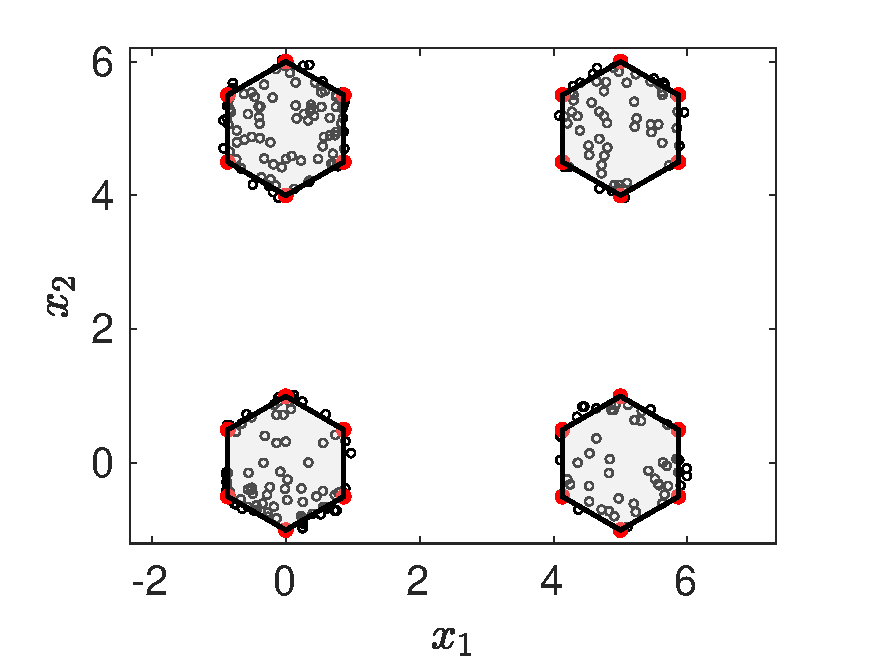
\includegraphics[width=\linewidth]{Section5/dim2/PS/NSGAII}
    \caption{NSGA-II}
    \end{subfigure}
    \begin{subfigure}[b]{.22\textwidth}
    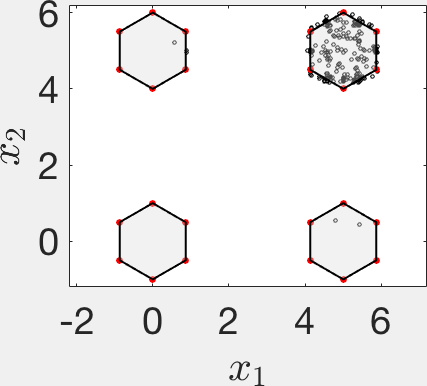
\includegraphics[width=\linewidth]{Section5/dim2/PS/NSGAIII}
    \caption{NSGA-III}
    \end{subfigure}
    
    \begin{subfigure}[b]{.22\textwidth}
    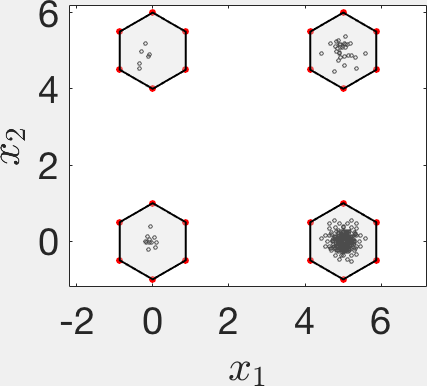
\includegraphics[width=\linewidth]{Section5/dim2/PS/MOEAD_TCH}
    \caption{MOEA/D-TCH}
    \end{subfigure}
    \begin{subfigure}[b]{.22\textwidth}
    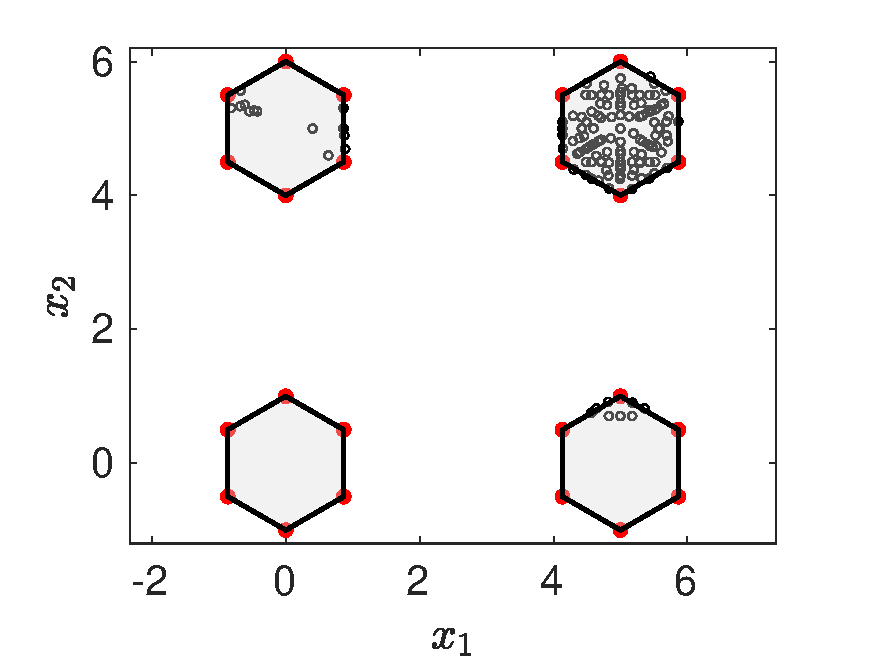
\includegraphics[width=\linewidth]{Section5/dim2/PS/MOEAD_PBI}
    \caption{MOEA/D-PBI}
    \end{subfigure}
    
    \begin{subfigure}[b]{.22\textwidth}
    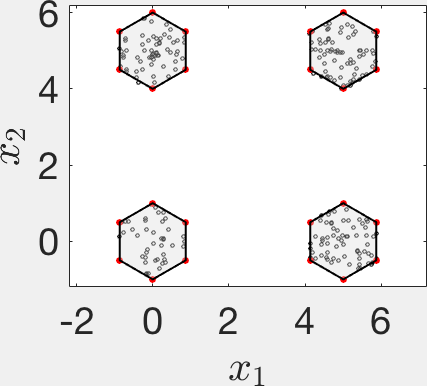
\includegraphics[width=\linewidth]{Section5/dim2/PS/IBEA}
    \caption{IBEA}
    \end{subfigure}
    \begin{subfigure}[b]{.22\textwidth}
    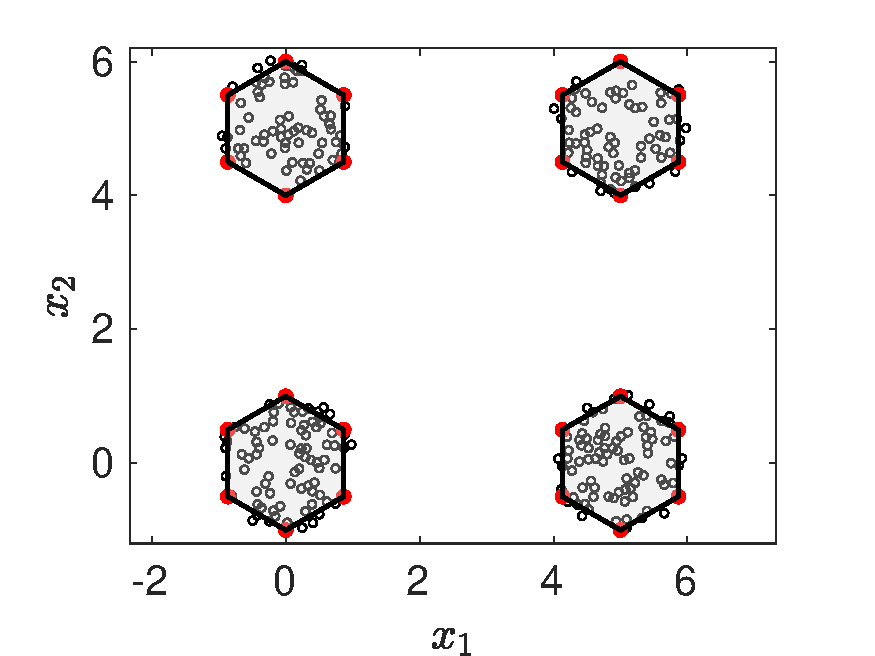
\includegraphics[width=\linewidth]{Section5/dim2/PS/SPEA2}
    \caption{SPEA2}
    \end{subfigure}
    \caption{Simulation results of MOEAs on Multi-Polygon test problem with $D=2$.}
    \label{fig: MOEAs PS dim=2}
\end{figure}

\begin{figure}[htbp]
    \centering
    \begin{subfigure}[b]{.22\textwidth}
    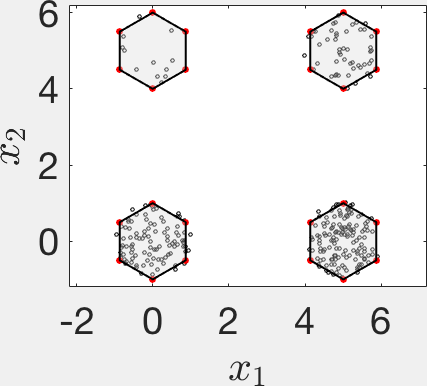
\includegraphics[width=\linewidth]{Section5/dim2/PS/DNEA}
    \caption{DNEA}
    \end{subfigure}
    \begin{subfigure}[b]{.22\textwidth}
    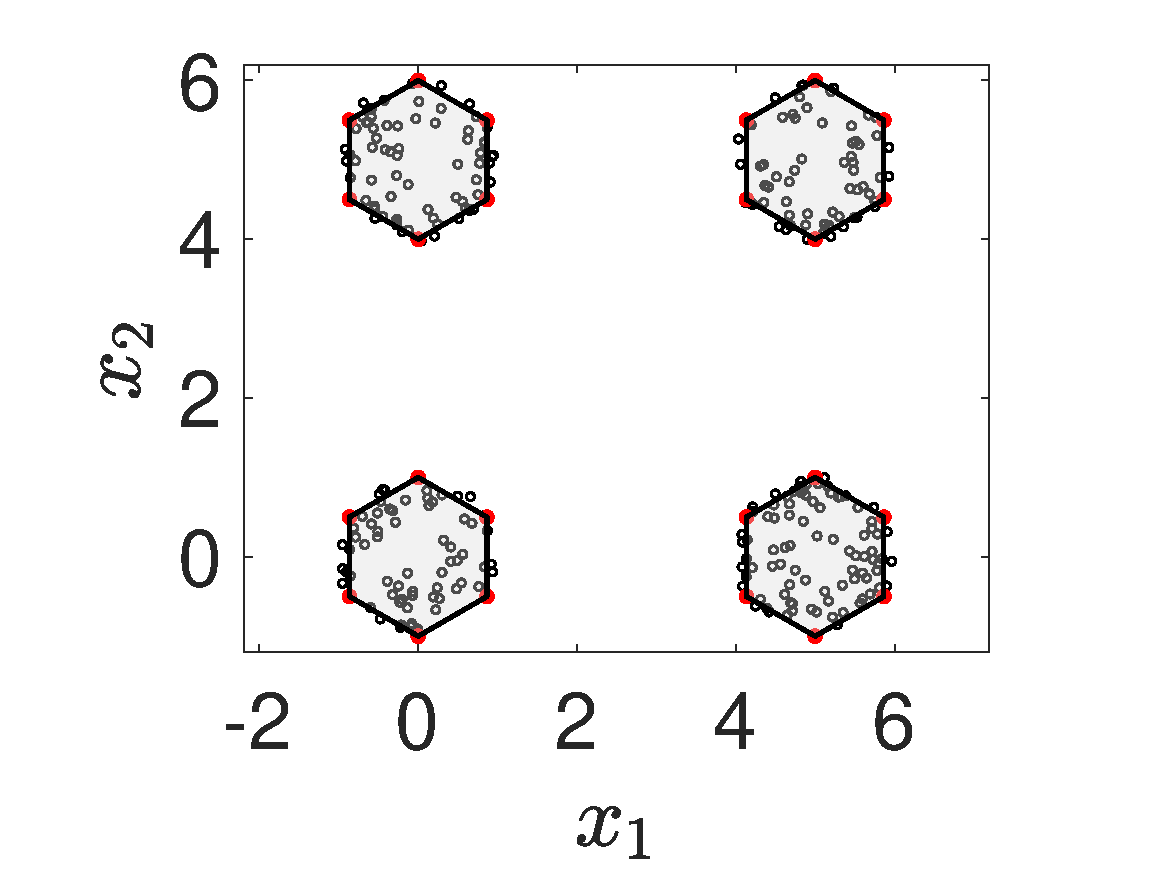
\includegraphics[width=\linewidth]{Section5/dim2/PS/MO_Ring_PSO_SCD}
    \caption{MO\_Ring\_PSO\_SCD}
    \end{subfigure}
    
    \begin{subfigure}[b]{.22\textwidth}
    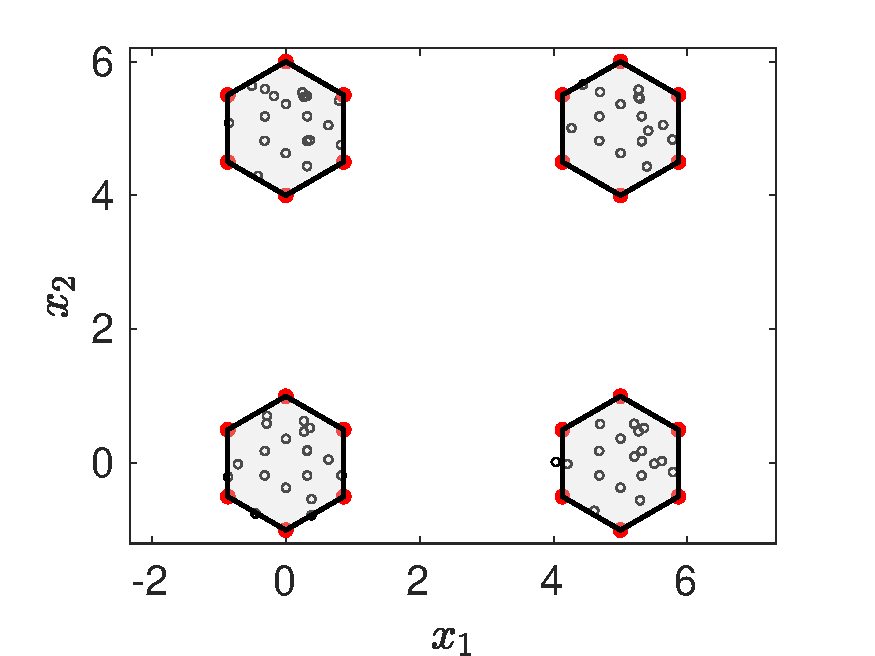
\includegraphics[width=\linewidth]{Section5/dim2/PS/MOEADAD}
    \caption{MOEA/D-AD}
    \end{subfigure}
    \begin{subfigure}[b]{.22\textwidth}
    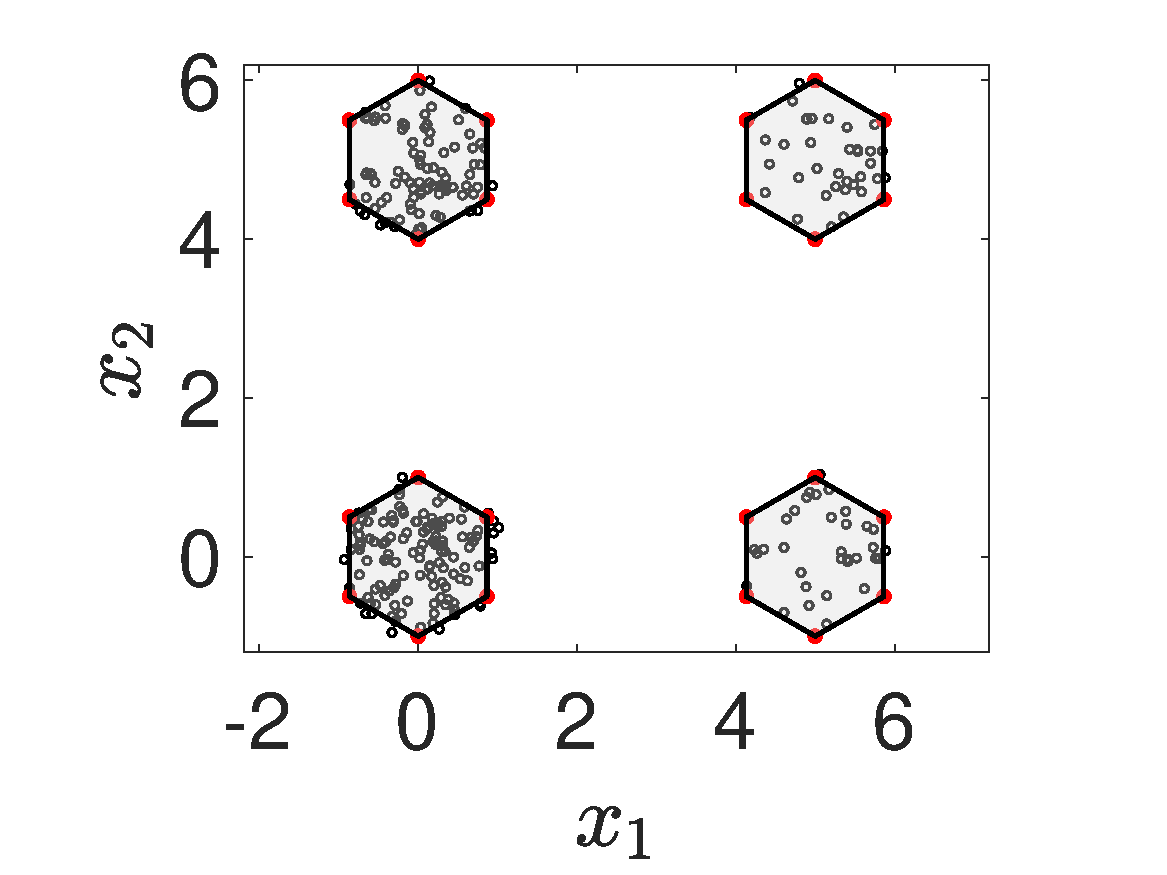
\includegraphics[width=\linewidth]{Section5/dim2/PS/OmniOptimizer}
    \caption{Omni-optimizer}
    \end{subfigure}
    \caption{Simulation results of MMEAs on Multi-Polygon test problem with $D=2$.}
    \label{fig: MMEAs PS dim=2}
\end{figure}

Figure \ref{fig: MOEAs PS dim=2} and \ref{fig: MMEAs PS dim=2} show the simulation results of MOEAs and MMEAs when $D=2$. It can be seen that the performance of MOEA/D and NSGA-III is worst than other algorithms. When $D=2$, all algorithms except MOEA/D and NSGA-III can obtain a good coverage of the true Pareto sets. It is worth mentioning that, because the deletion mechanism is introduced in MOEA/D-AD, the number of solutions obtained is smaller than others. 

As discussed in section \ref{Difficulties Analysis}, we pointed out that the performance of MOEAs on the MMOPs should be very poor. However, the experimental results here are inconsistent with this proposition. In order to figure out the reason, we divided the plane into four parts, and mark them as area 1\textasciitilde 4 in counterclockwise order as show in figure \ref{fig: Alleles}. Then, after every 500 evaluations(denoted as epoch), the number of solutions lie in each area is recorded. In addition, the IGD value of each epoch is also recorded to show the evolutionary progress. 

%% dim = 2 Diversity Plot
\begin{figure}[htbp]
    \centering
    \begin{subfigure}[b]{.22\textwidth}
    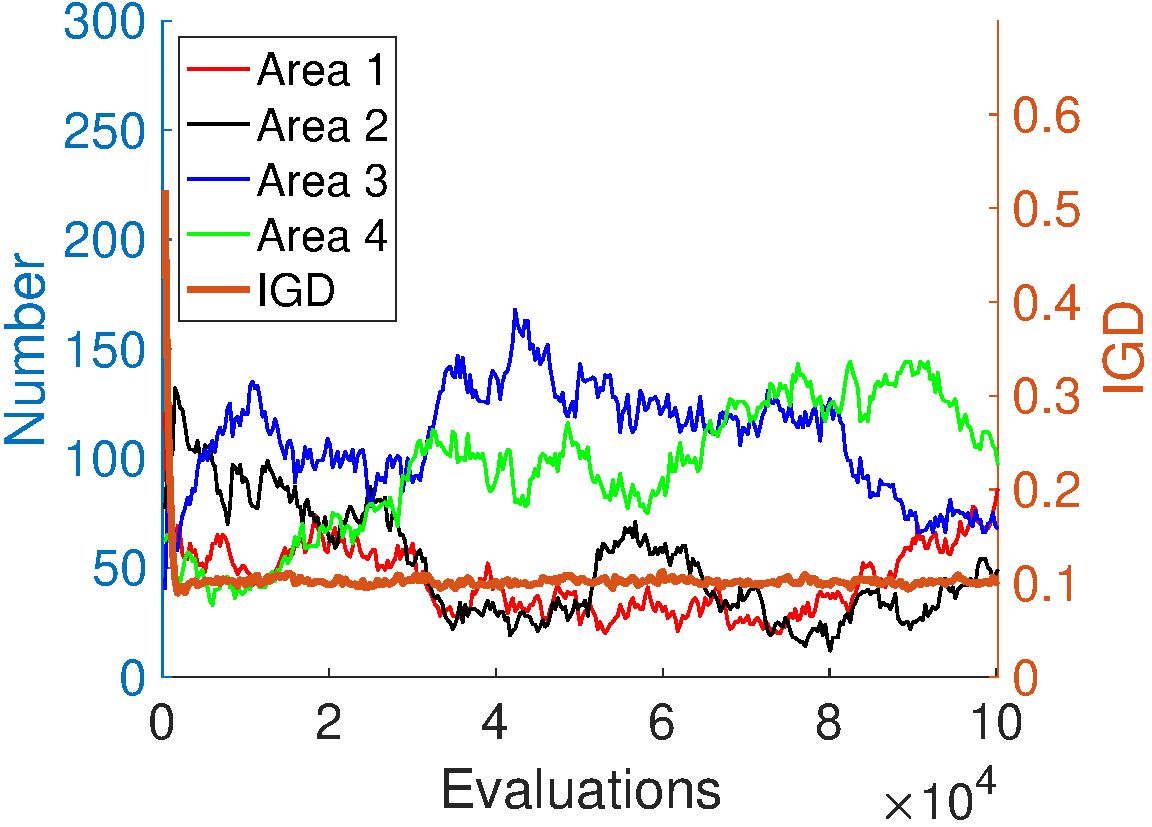
\includegraphics[width=\linewidth]{Section5/dim2/Diversity/NSGAII}
    \caption{NSGA-II}
    \end{subfigure}
    \begin{subfigure}[b]{.22\textwidth}
    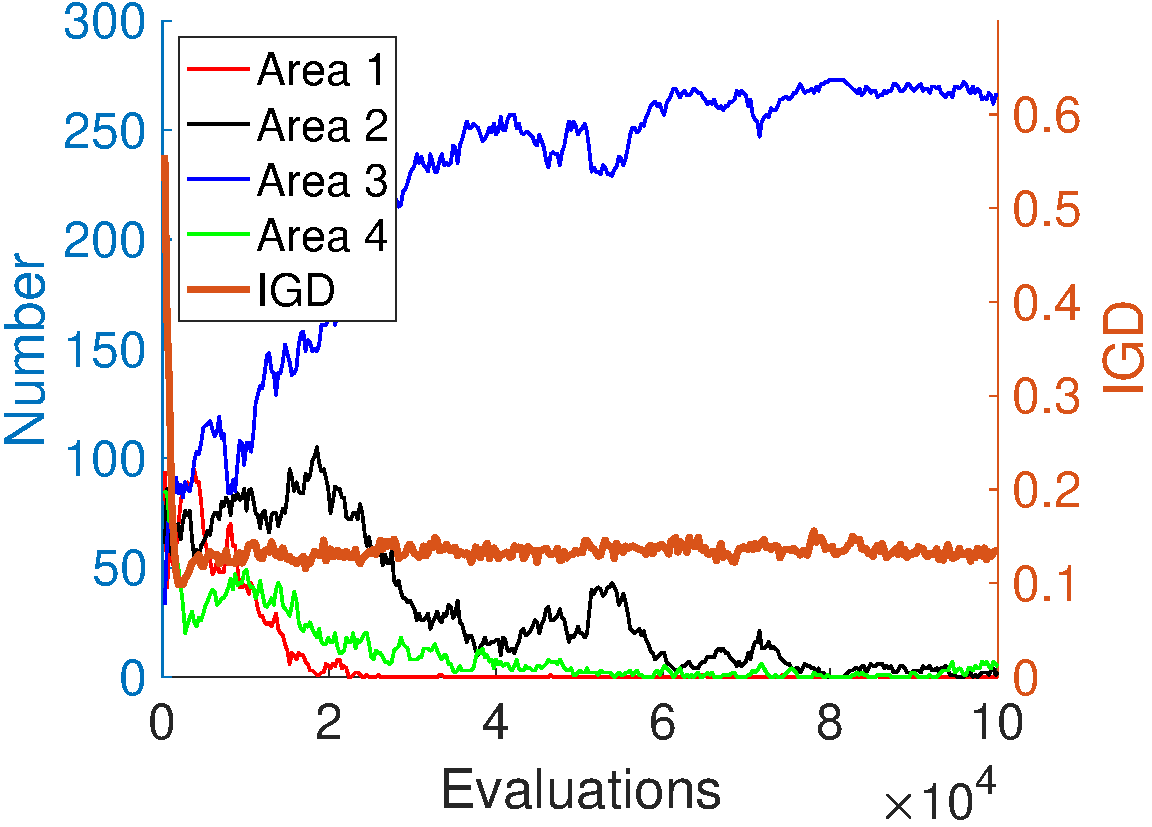
\includegraphics[width=\linewidth]{Section5/dim2/Diversity/NSGAIII}
    \caption{NSGA-III}
    \label{fig: NSGA-III Diversity dim=2}
    \end{subfigure}
    
    
    \begin{subfigure}[b]{.22\textwidth}
    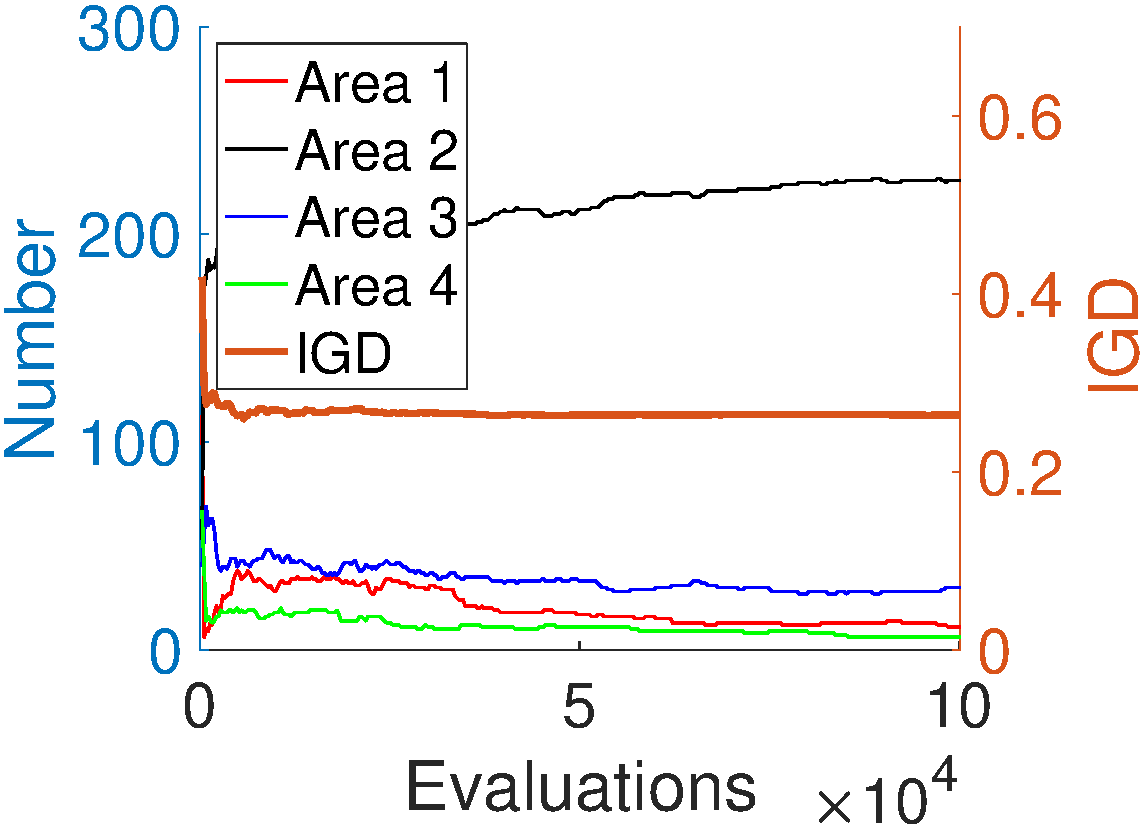
\includegraphics[width=\linewidth]{Section5/dim2/Diversity/MOEAD_TCH}
    \caption{MOEA/D-TCH}
    \label{fig: MOEA/D-TCH Diversity dim=2}
    \end{subfigure}
    \begin{subfigure}[b]{.22\textwidth}
    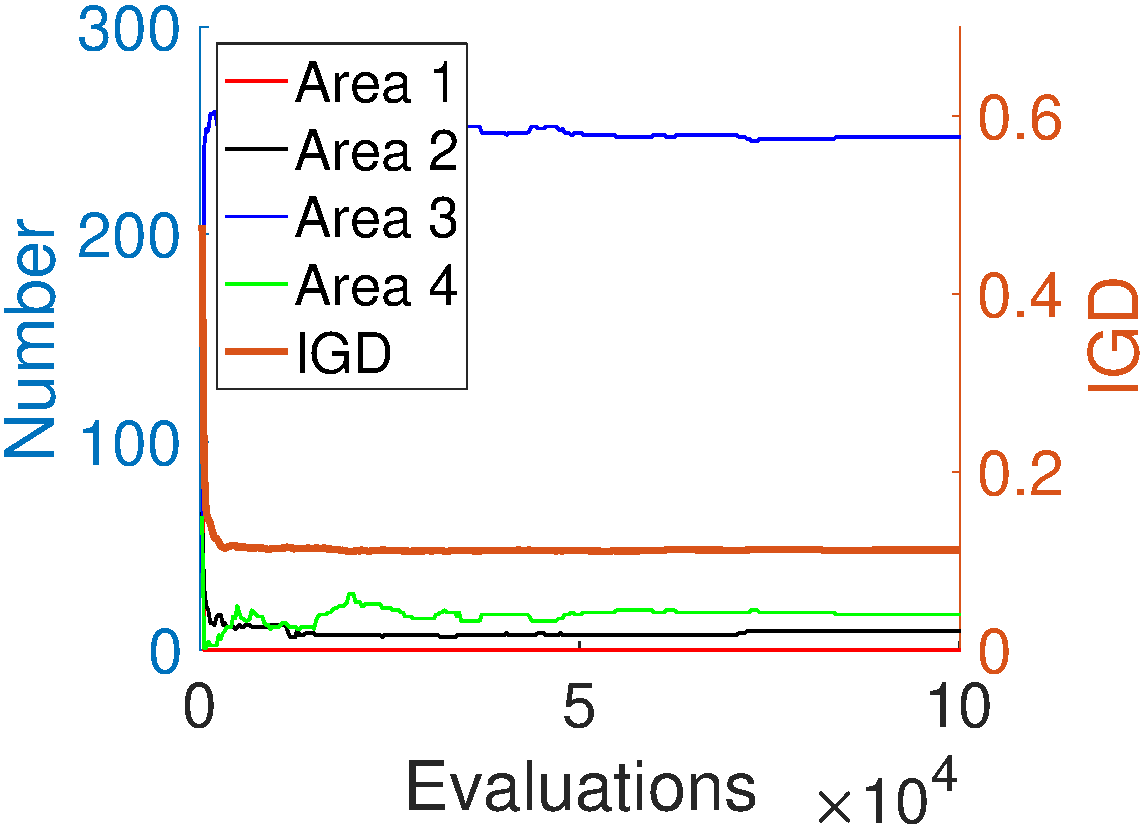
\includegraphics[width=\linewidth]{Section5/dim2/Diversity/MOEAD_PBI}
    \caption{MOEA/D-PBI}
    \label{fig: MOEA/D-PBI Diversity dim=2}
    \end{subfigure}
    
    \begin{subfigure}[b]{.22\textwidth}
    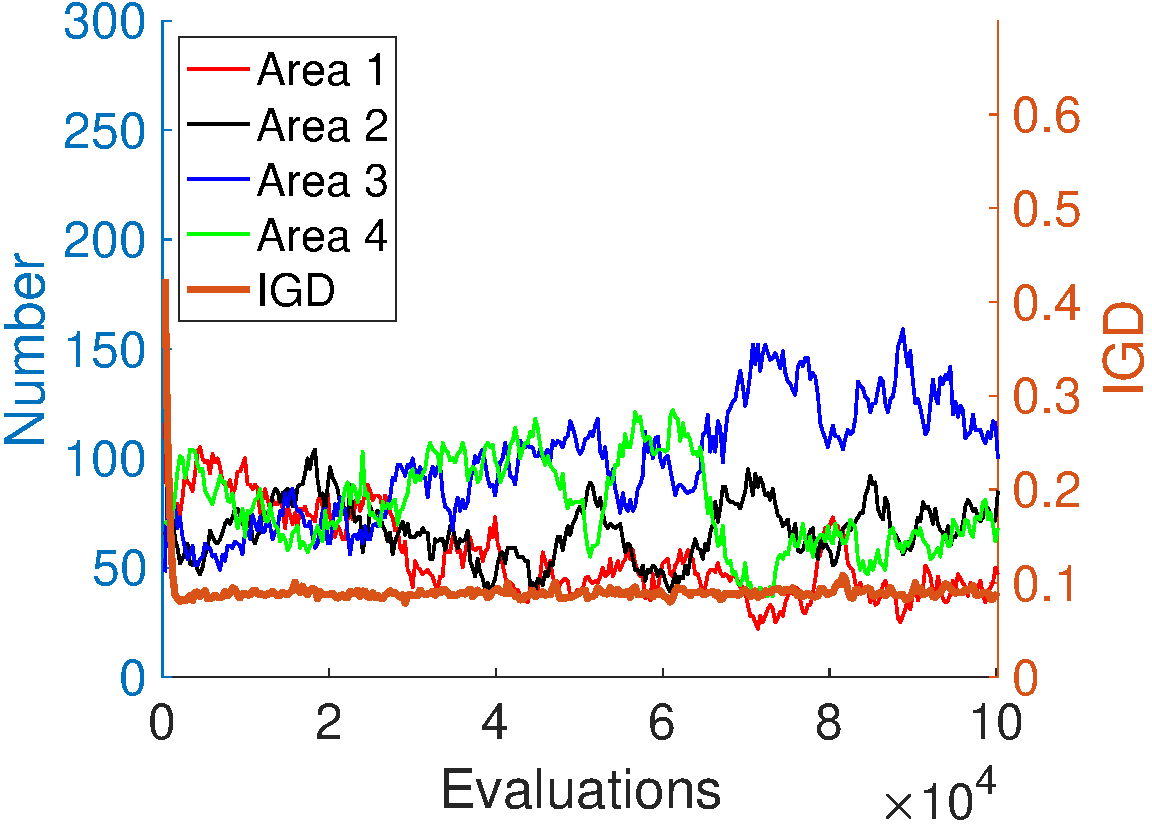
\includegraphics[width=\linewidth]{Section5/dim2/Diversity/IBEA}
    \caption{IBEA}
    \end{subfigure}
    \begin{subfigure}[b]{.22\textwidth}
    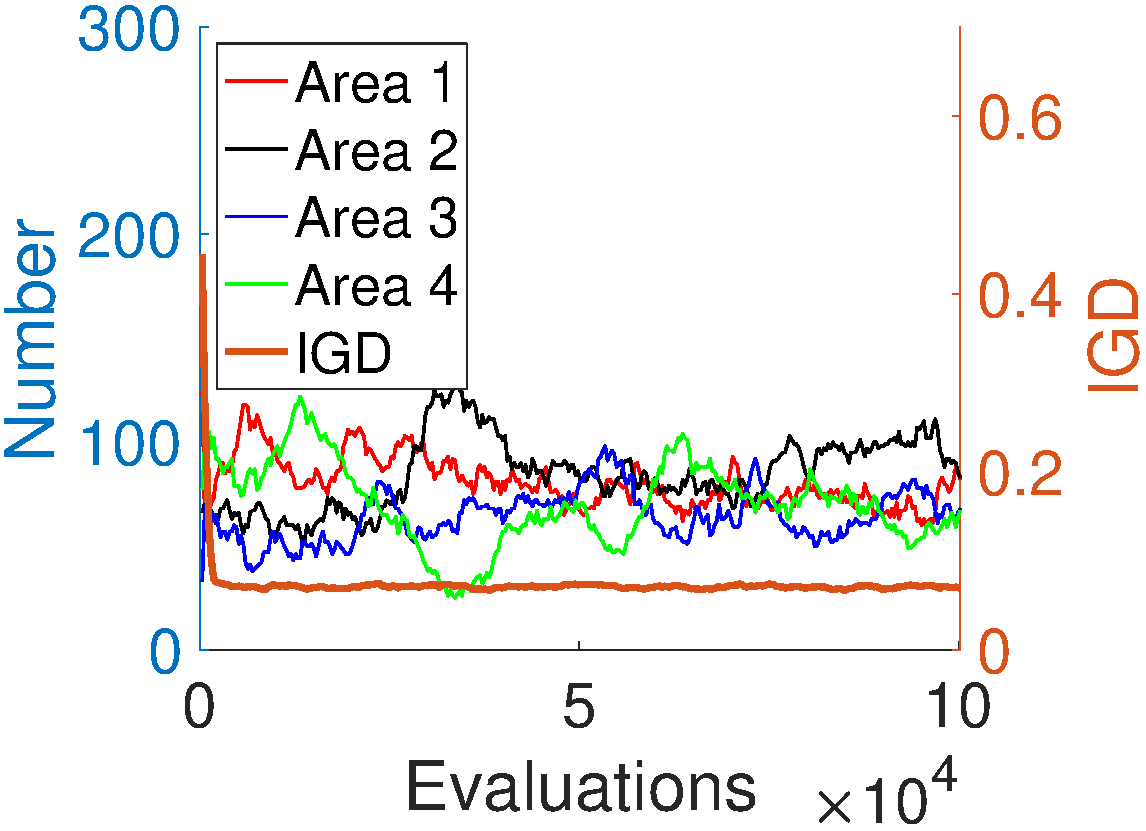
\includegraphics[width=\linewidth]{Section5/dim2/Diversity/SPEA2}
    \caption{SPEA2}
    \end{subfigure}
    \caption{Solution distribution and IGD value of MOEAs on Multi-Polygon test problem with $D=2$.}
    \label{fig: MOEAs Diversity dim=2}
\end{figure}

\begin{figure}[htbp]
    \centering
    \begin{subfigure}[b]{.22\textwidth}
    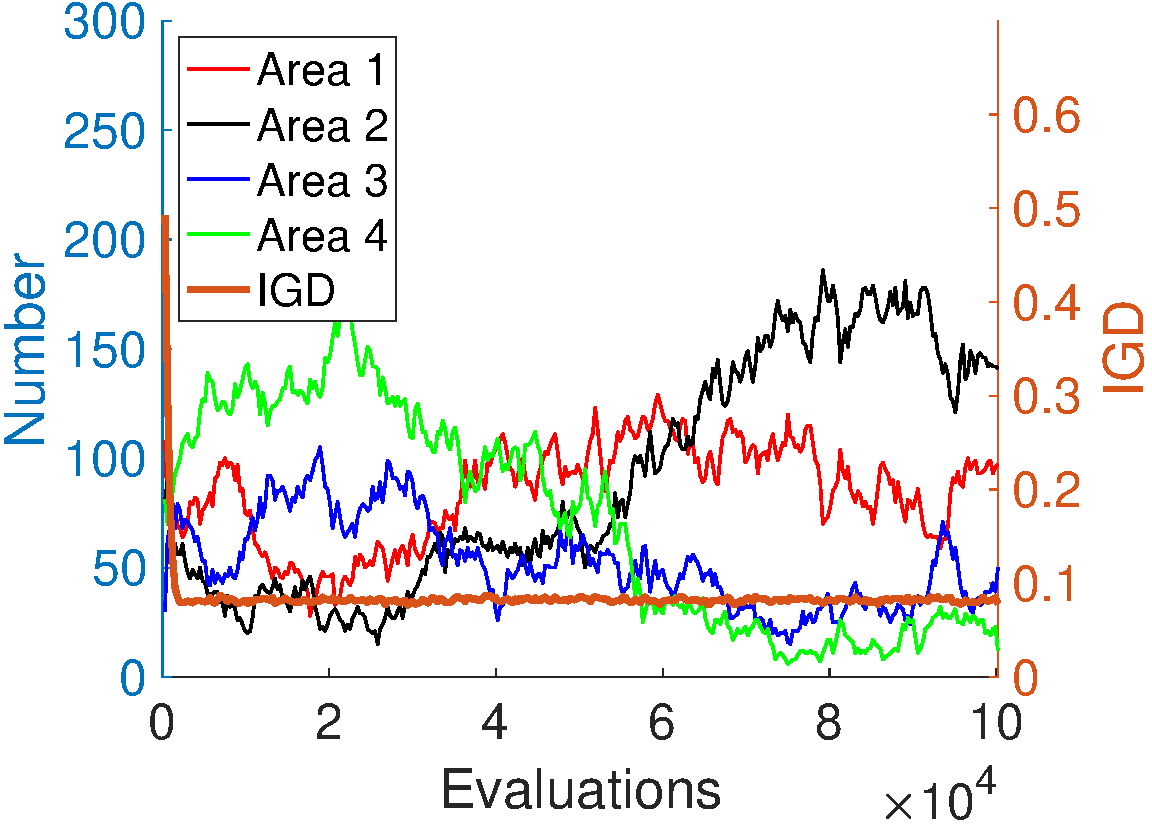
\includegraphics[width=\linewidth]{Section5/dim2/Diversity/DNEA}
    \caption{DNEA}
    \end{subfigure}
    \begin{subfigure}[b]{.22\textwidth}
    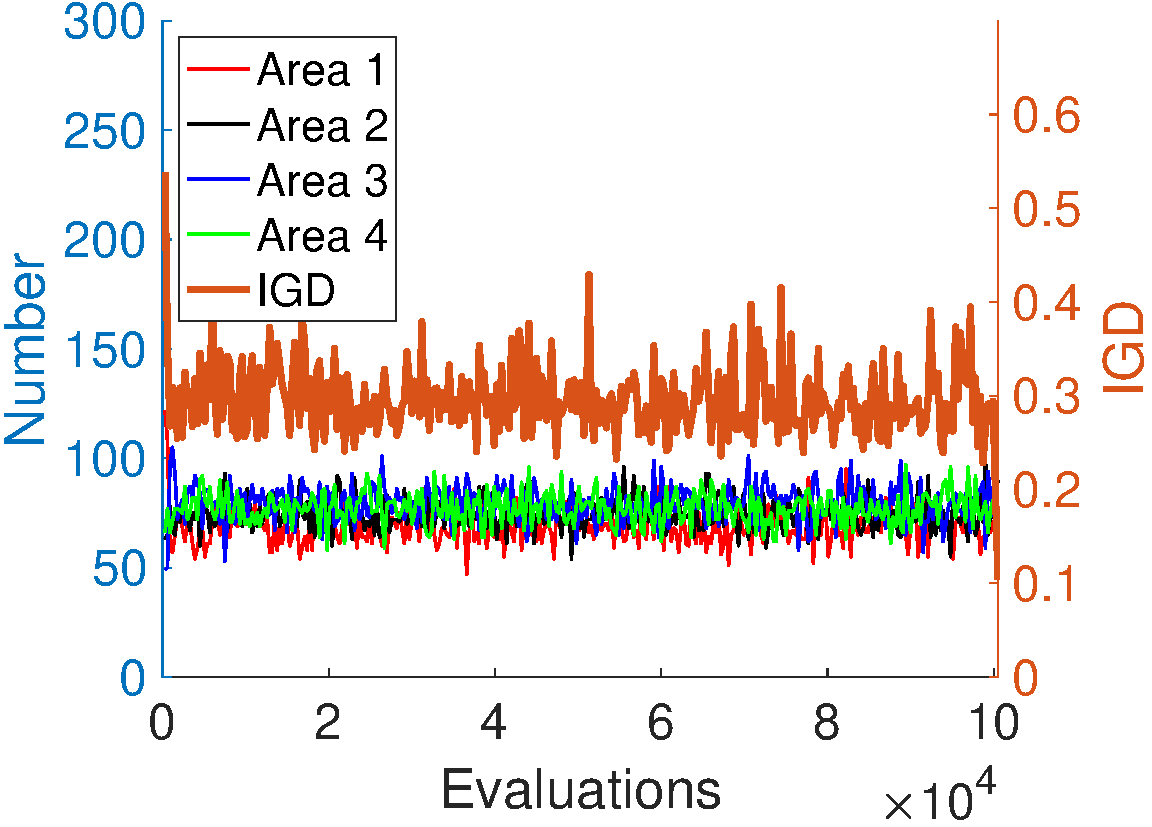
\includegraphics[width=\linewidth]{Section5/dim2/Diversity/MO_Ring_PSO_SCD}
    \caption{MO\_Ring\_PSO\_SCD}
    \end{subfigure}
    
    \begin{subfigure}[b]{.22\textwidth}
    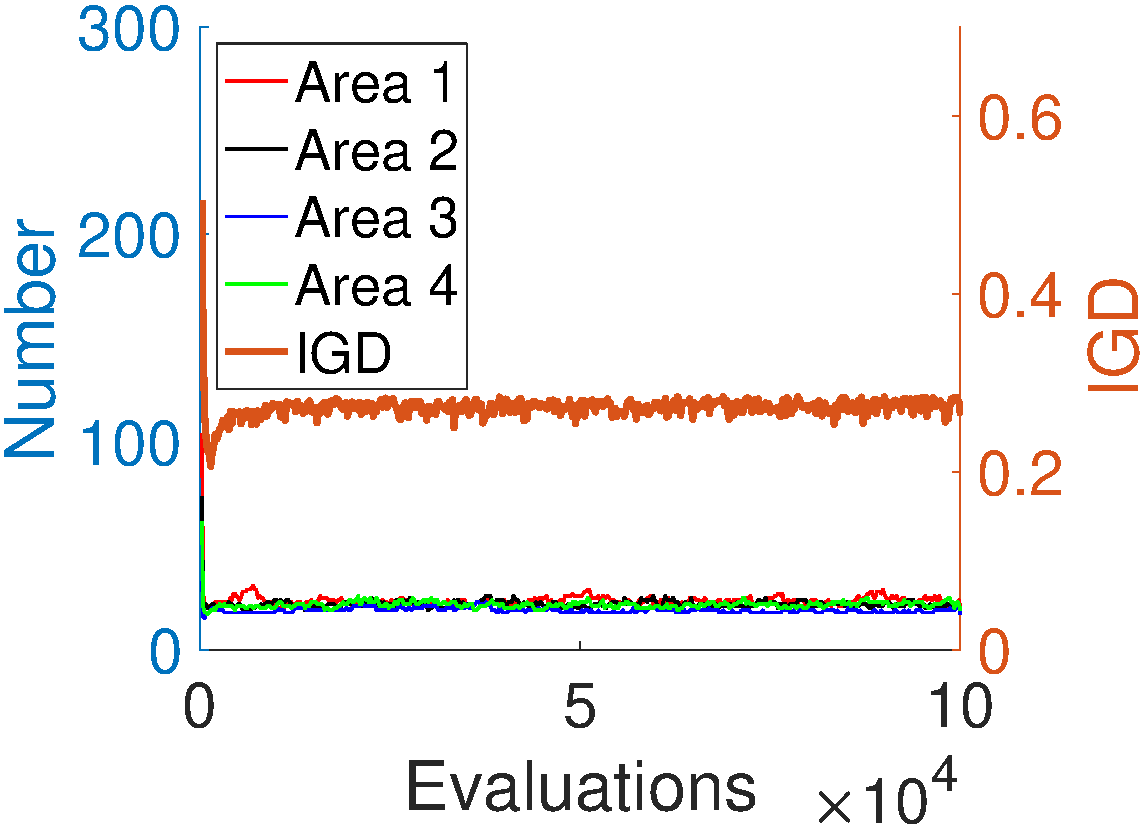
\includegraphics[width=\linewidth]{Section5/dim2/Diversity/MOEADAD}
    \caption{MOEA/D-AD}
    \end{subfigure}
    \begin{subfigure}[b]{.22\textwidth}
    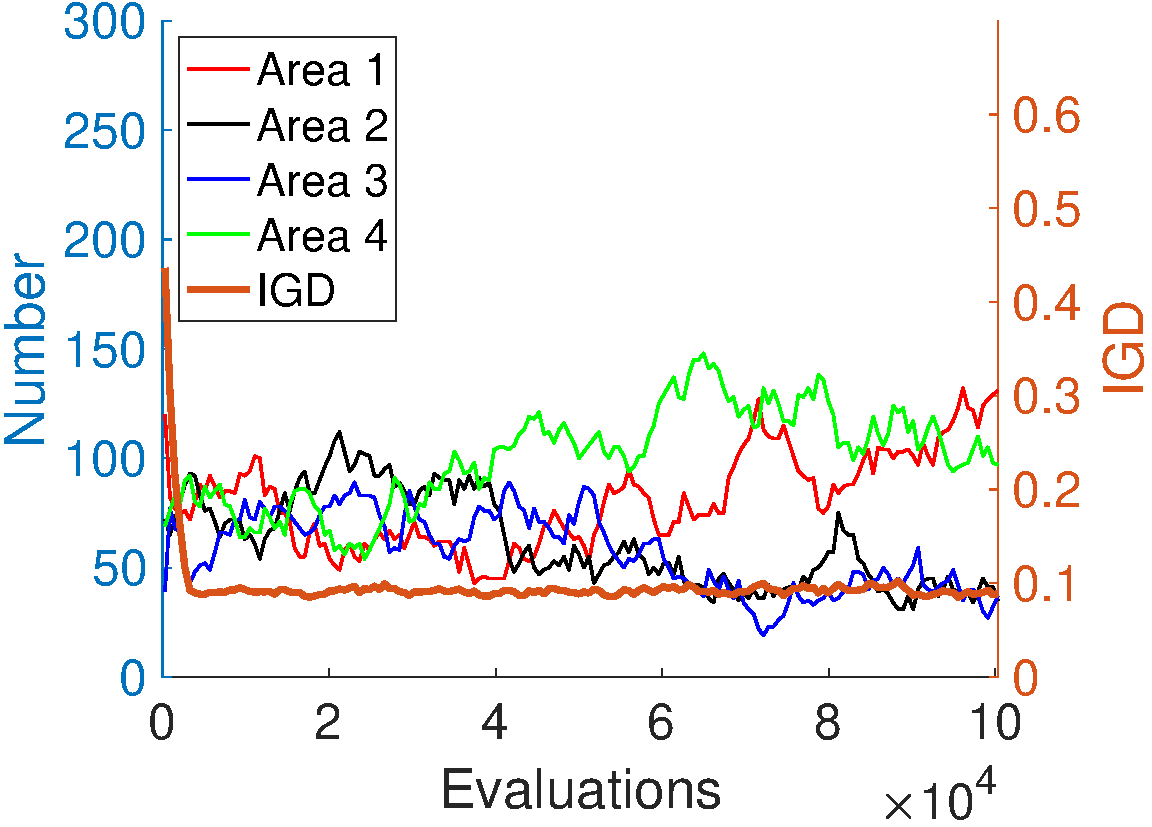
\includegraphics[width=\linewidth]{Section5/dim2/Diversity/OmniOptimizer}
    \caption{Omni-optimizer}
    \end{subfigure}
    \caption{Solution distribution and IGD value of MMEAs on Multi-Polygon test problem with $D=2$.}
    \label{fig: MMEAs PS dim=2}
\end{figure}

Figure \ref{fig: MOEAs Diversity dim=2} and \ref{fig: MMEAs PS dim=2} show the solution distribution and IGD value at each epoch for MOEAs and MMEAs respectively. According to figure \ref{fig: MOEAs Diversity dim=2}, for MOEAs which perform good when $D=2$, the number of solutions in each area establish a "dynamic balance". As shown in figure \ref{fig: SBX crossover case 2}, by applying SBX crossover to two solutions in diagonal area will significantly improve the diversity in decision space. When the number of solutions in diagonal area is very close, a dynamic balance is formed. When the number solution is one area is much larger than it's diagonal area, SBX crossover cannot provide enough variety to counter the effect of genetic drift, therefore all equivalent solutions(alleles) will disappear, i.e. only solutions in single polygon left. Take NSGA-III as an example, in figure \ref{fig: NSGA-III Diversity dim=2}, at about $10^4$ evaluations, the population becomes mature and the diversity of solution is good. However, since area 3 has much more solutions than others, solutions in other area quickly disappear. This kind of figures may also help to explain the poor performance of MOEA/D. It can bee seen from figure \ref{fig: MOEA/D-TCH Diversity dim=2} and \ref{fig: MOEA/D-PBI Diversity dim=2} that MOEA/D focus it's search in a small area in decision space at the young stage of evolution. We can conclude that MOEA/D lost it's diversity in decision space because of it's environmental selection mechanism.

For MMEAs, the situation that one allele dominate other never happen when $D=2$, all of them can establish dynamic balance. Diversity maintenance strategies used in MMEAs are effective in this case.

Following same manner, we examine the case when $D=4$. The 2-d projection of the final population is shown in figure \ref{fig: MOEAs PS dim=4} and \ref{fig: MMEAs PS dim=4}. The simulation results show that it is more difficult to obtain good Pareto sets coverage in decision space. Most MOEAs only obtain solutions in one or two polygons. For MMEAs, MOEA/D-AD and MO\_Ring\_PSO\_SCD obtain satisfactory results but the performance of DNEA and Omni-optimizer is worse than our expectations. This shows that the adaptability of fitness sharing and crowding distance approach is not good.


%% dim = 4 PS plot 
\begin{figure}[htbp]
    \centering
    \begin{subfigure}[b]{.22\textwidth}
    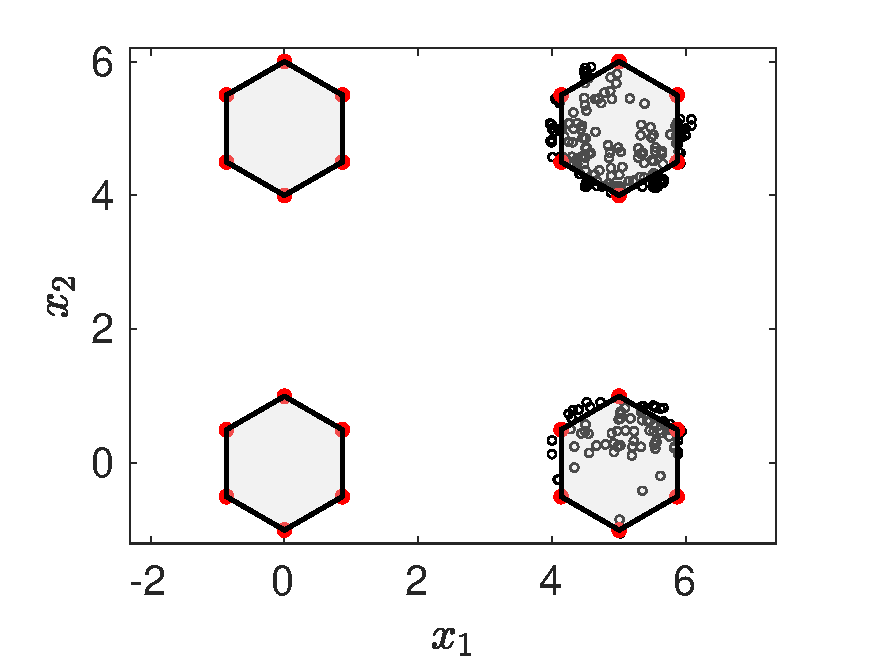
\includegraphics[width=\linewidth]{Section5/dim4/PS/NSGAII}
    \caption{NSGA-II}
    \end{subfigure}
    \begin{subfigure}[b]{.22\textwidth}
    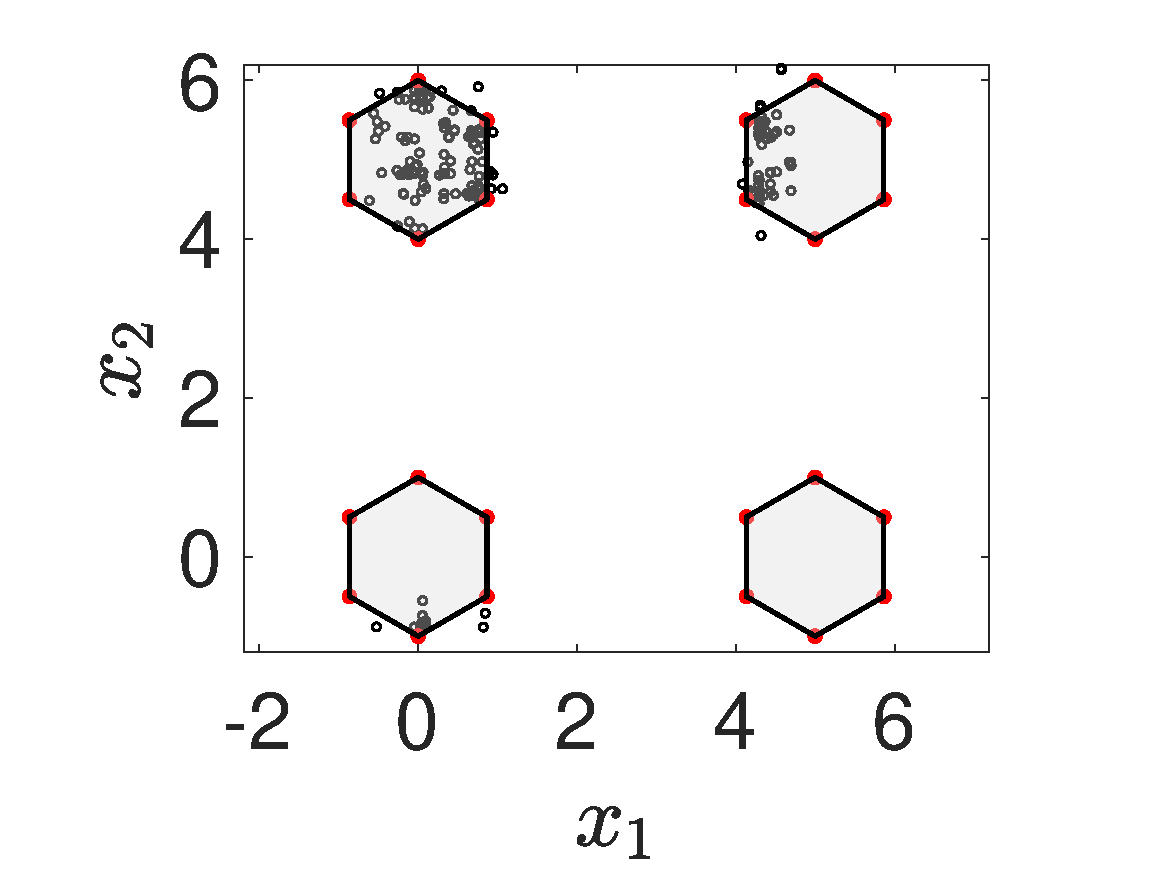
\includegraphics[width=\linewidth]{Section5/dim4/PS/NSGAIII}
    \caption{NSGA-III}
    \end{subfigure}
    
    \begin{subfigure}[b]{.22\textwidth}
    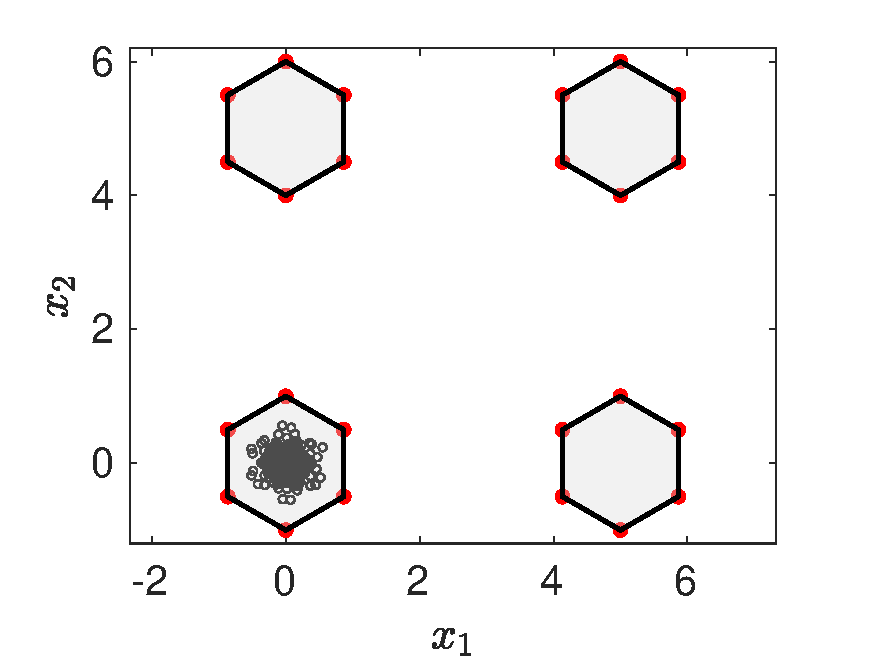
\includegraphics[width=\linewidth]{Section5/dim4/PS/MOEAD_TCH}
    \caption{MOEA/D-TCH}
    \end{subfigure}
    \begin{subfigure}[b]{.22\textwidth}
    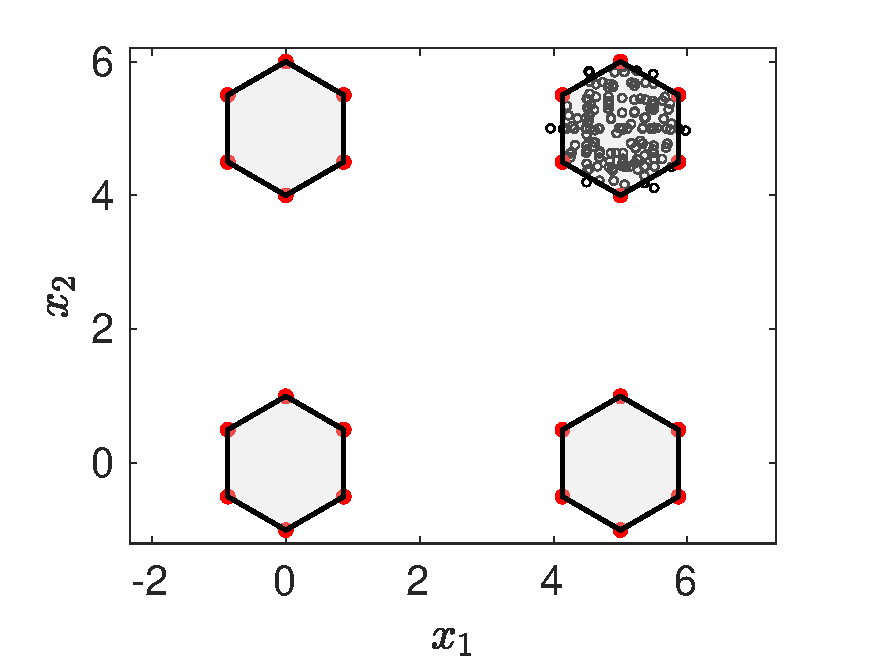
\includegraphics[width=\linewidth]{Section5/dim4/PS/MOEAD_PBI}
    \caption{MOEA/D-PBI}
    \end{subfigure}
    
    \begin{subfigure}[b]{.22\textwidth}
    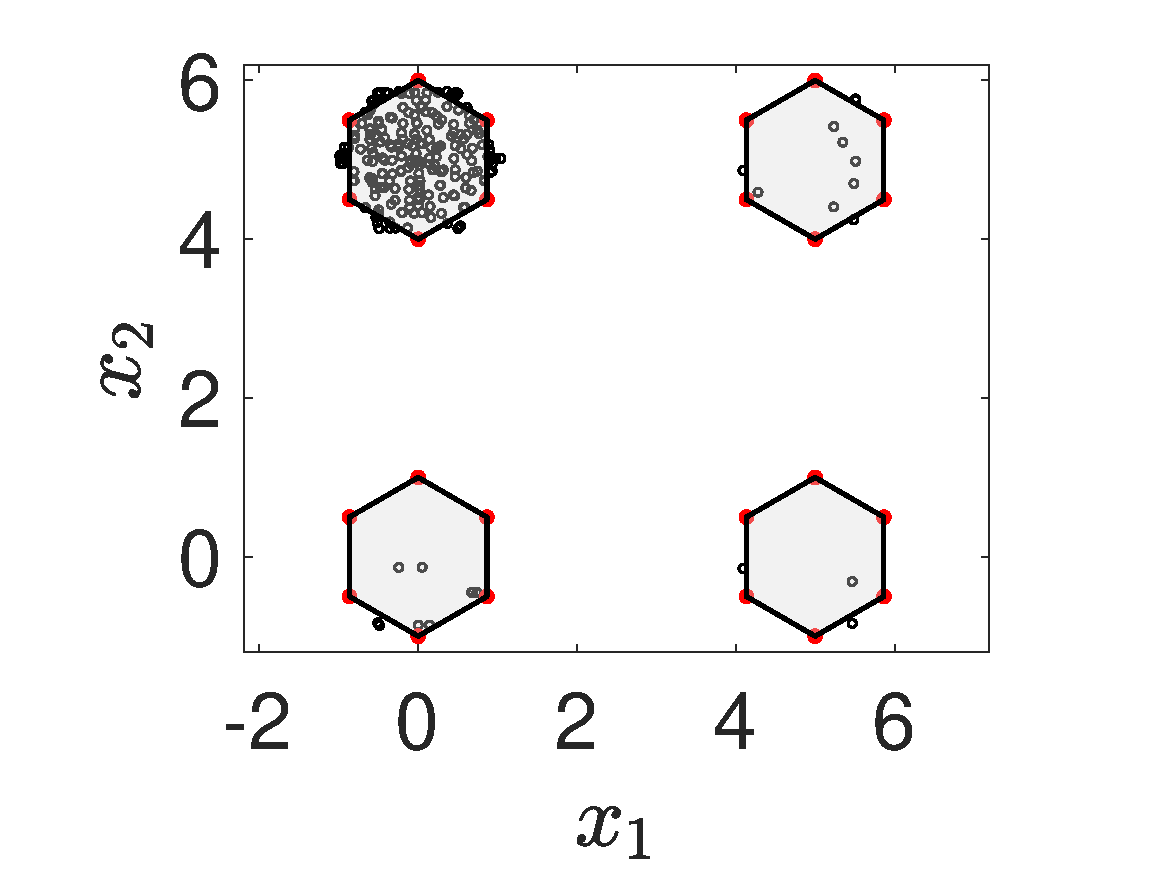
\includegraphics[width=\linewidth]{Section5/dim4/PS/IBEA}
    \caption{IBEA}
    \end{subfigure}
    \begin{subfigure}[b]{.22\textwidth}
    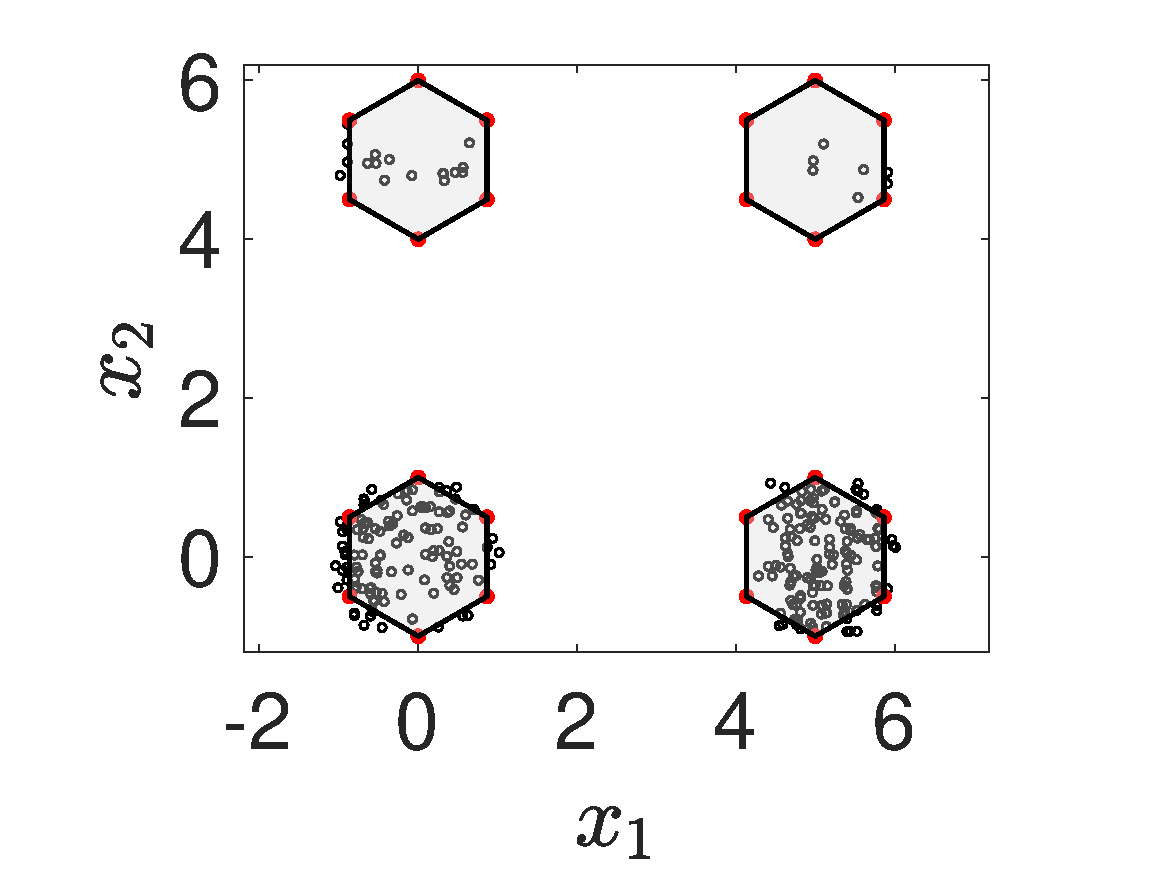
\includegraphics[width=\linewidth]{Section5/dim4/PS/SPEA2}
    \caption{SPEA2}
    \end{subfigure}
    \caption{Simulation results of MOEAs on Multi-Polygon test problem with $D=4$.}
    \label{fig: MOEAs PS dim=4}
\end{figure}

\begin{figure}[htbp]
    \centering
    \begin{subfigure}[b]{.22\textwidth}
    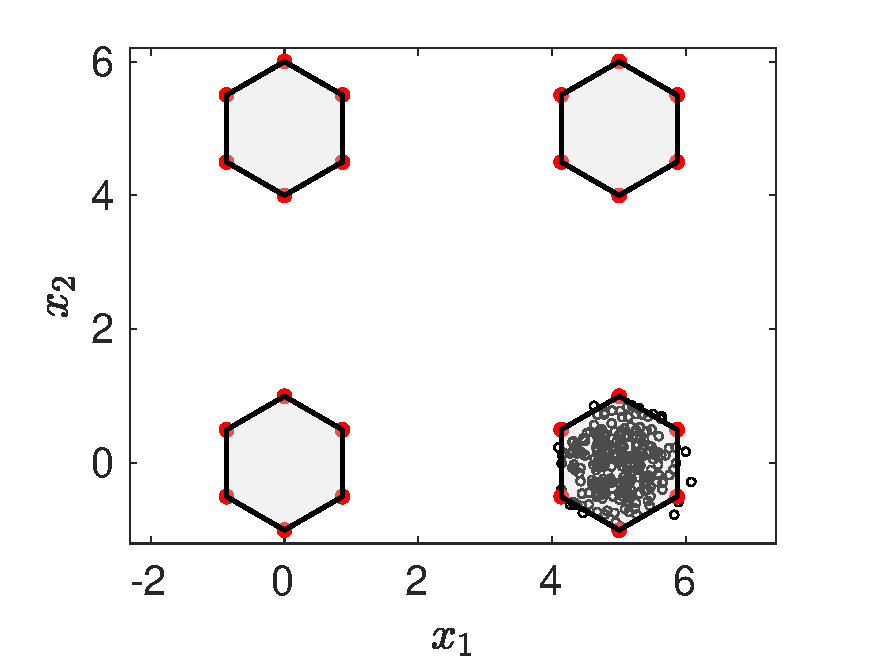
\includegraphics[width=\linewidth]{Section5/dim4/PS/DNEA}
    \caption{DNEA}
    \end{subfigure}
    \begin{subfigure}[b]{.22\textwidth}
    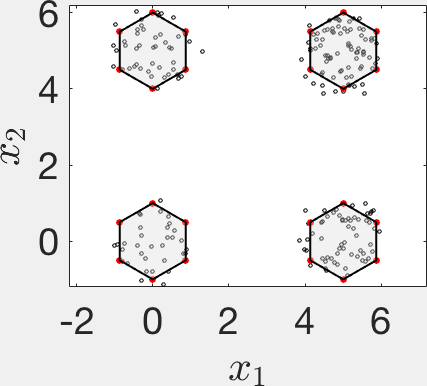
\includegraphics[width=\linewidth]{Section5/dim4/PS/MO_Ring_PSO_SCD}
    \caption{MO\_Ring\_PSO\_SCD}
    \end{subfigure}
    
    \begin{subfigure}[b]{.22\textwidth}
    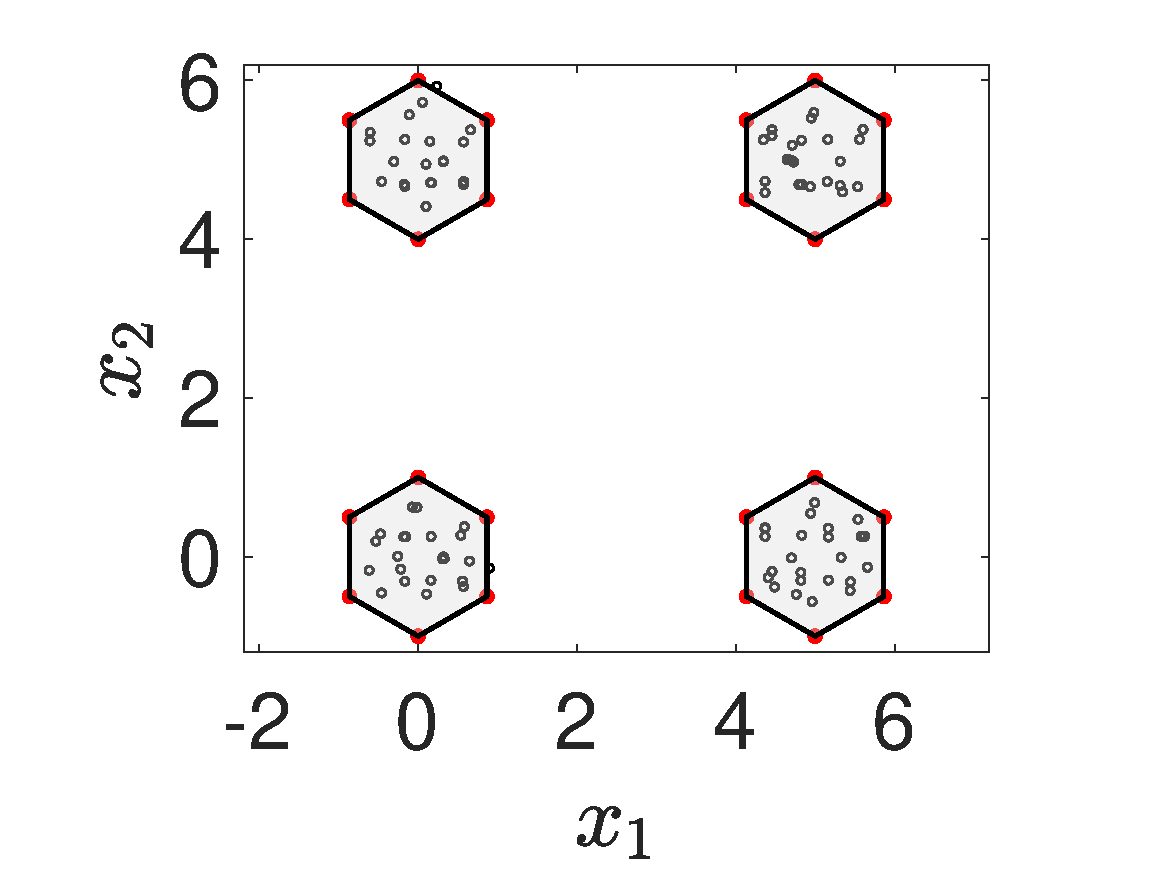
\includegraphics[width=\linewidth]{Section5/dim4/PS/MOEADAD}
    \caption{MOEA/D-AD}
    \end{subfigure}
    \begin{subfigure}[b]{.22\textwidth}
    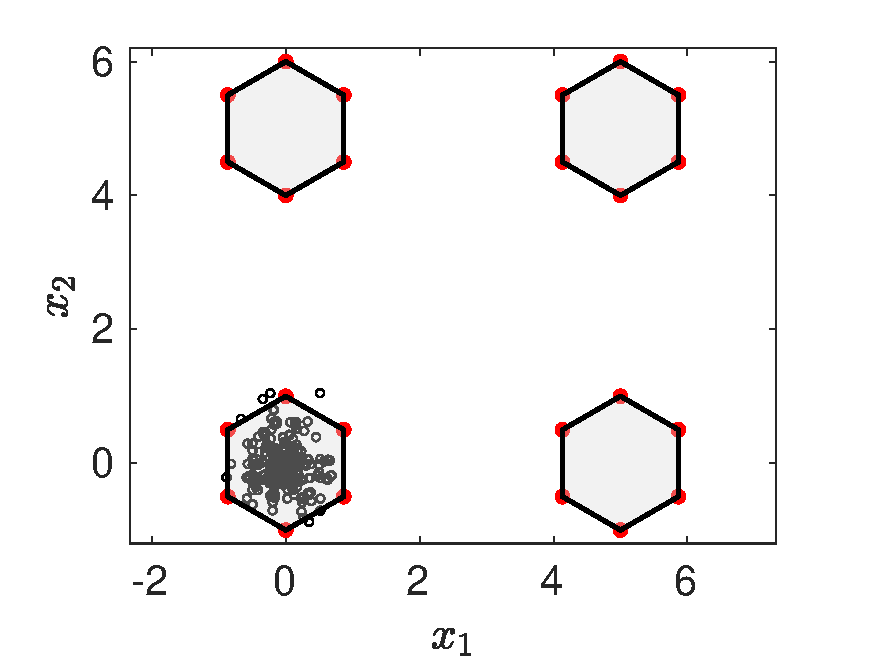
\includegraphics[width=\linewidth]{Section5/dim4/PS/OmniOptimizer}
    \caption{Omni-optimizer}
    \end{subfigure}
    \caption{Simulation results of MMEAs on Multi-Polygon test problem with $D=4$.}
    \label{fig: MMEAs PS dim=4}
\end{figure}

We also examine the solution distribution in the evolution process. According to figure \ref{fig: MOEAs Diversity dim=4} and \ref{fig: MMEAs Diversity dim=4}, we can see that when $D=4$, it is harder to establish dynamic balance than $D=2$ and the change of the number of solutions in each area is small.
%% dim = 4 Diversity Plot
\begin{figure}[htbp]
    \centering
    \begin{subfigure}[b]{.22\textwidth}
    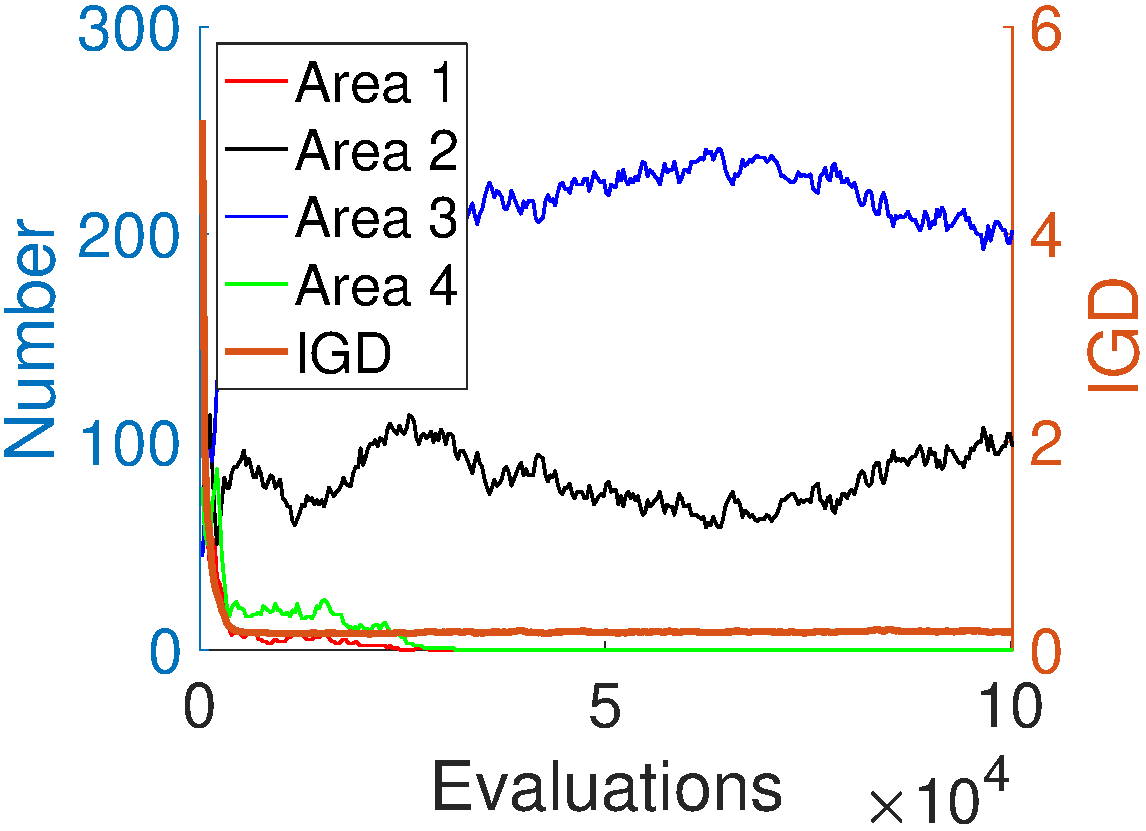
\includegraphics[width=\linewidth]{Section5/dim4/Diversity/NSGAII}
    \caption{NSGA-II}
    \end{subfigure}
    \begin{subfigure}[b]{.22\textwidth}
    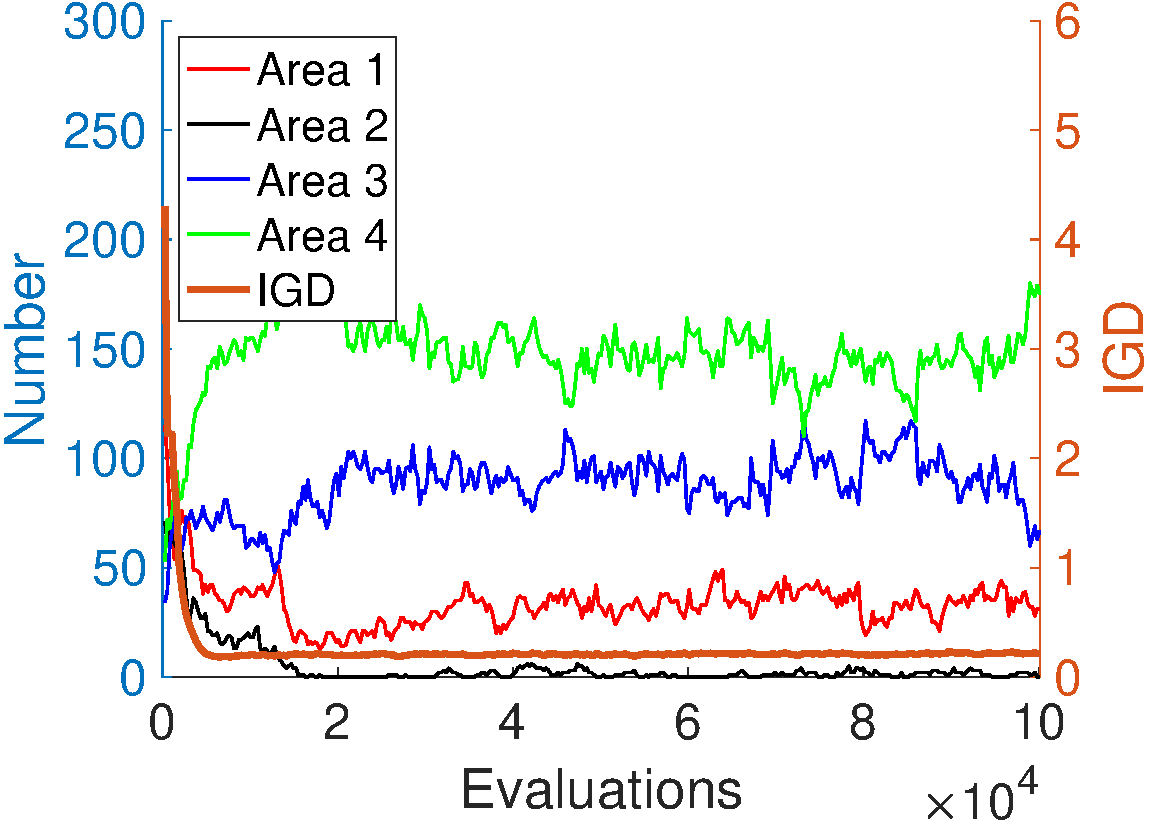
\includegraphics[width=\linewidth]{Section5/dim4/Diversity/NSGAIII}
    \caption{NSGA-III}
    \end{subfigure}
    
    
    \begin{subfigure}[b]{.22\textwidth}
    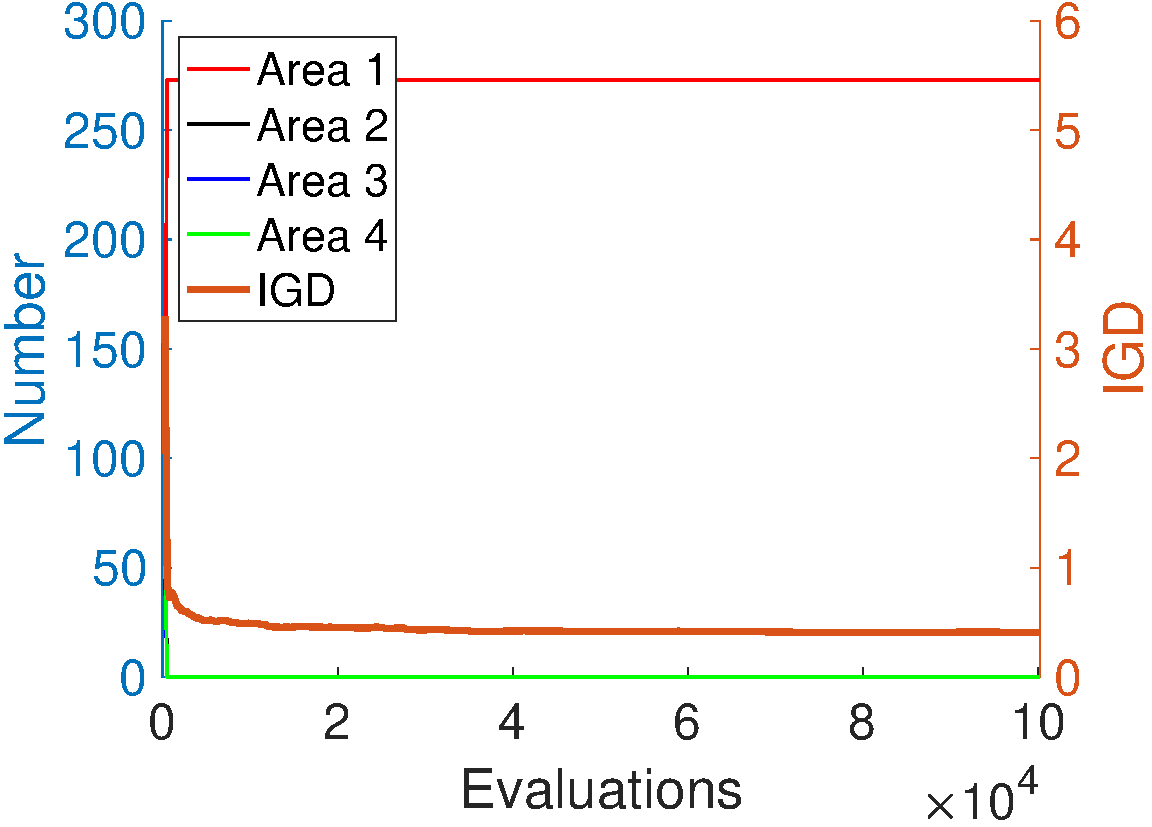
\includegraphics[width=\linewidth]{Section5/dim4/Diversity/MOEAD_TCH}
    \caption{MOEA/D-TCH}
    \end{subfigure}
    \begin{subfigure}[b]{.22\textwidth}
    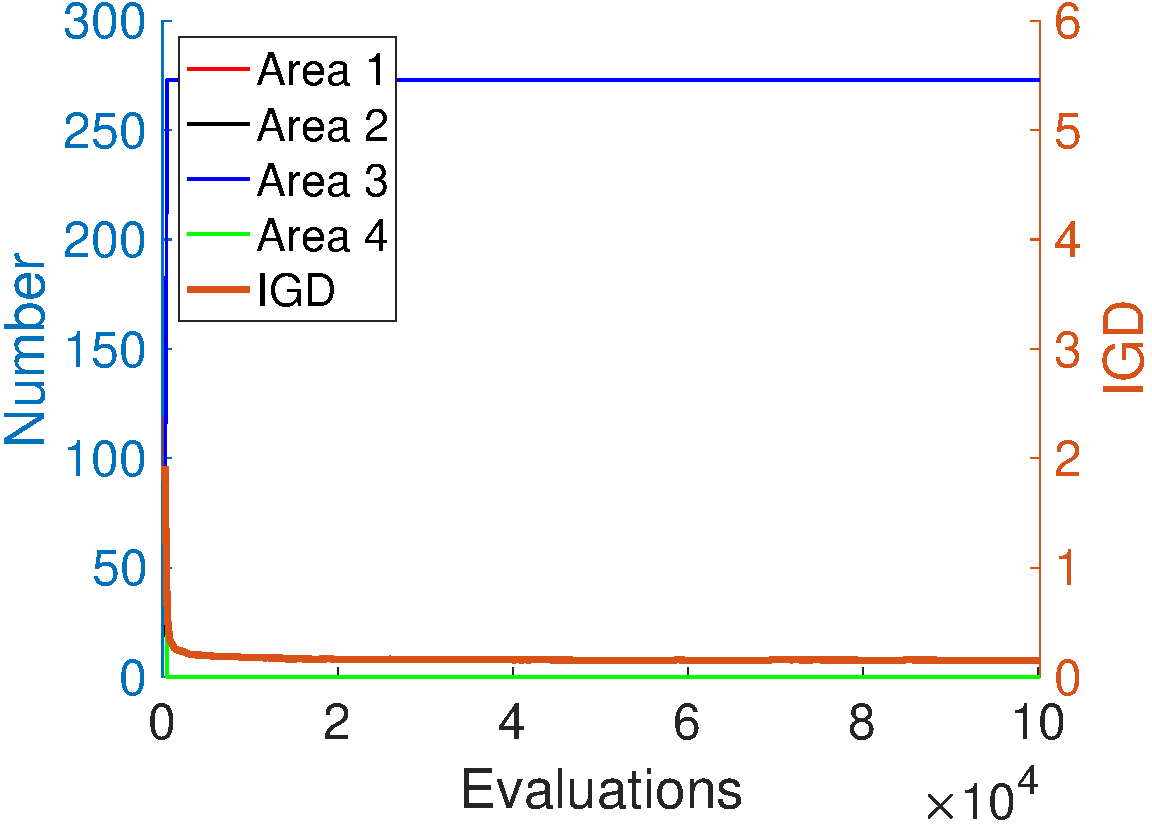
\includegraphics[width=\linewidth]{Section5/dim4/Diversity/MOEAD_PBI}
    \caption{MOEA/D-PBI}
    \end{subfigure}
    
    \begin{subfigure}[b]{.22\textwidth}
    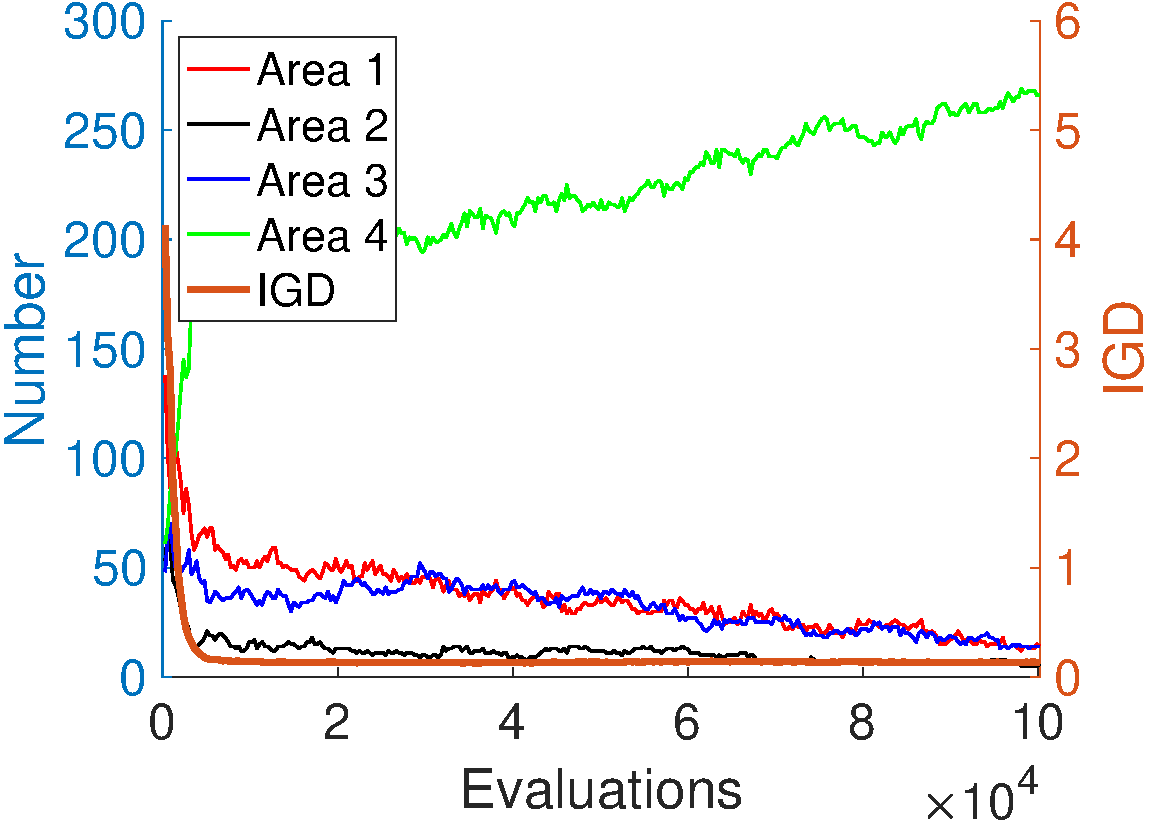
\includegraphics[width=\linewidth]{Section5/dim4/Diversity/IBEA}
    \caption{IBEA}
    \end{subfigure}
    \begin{subfigure}[b]{.22\textwidth}
    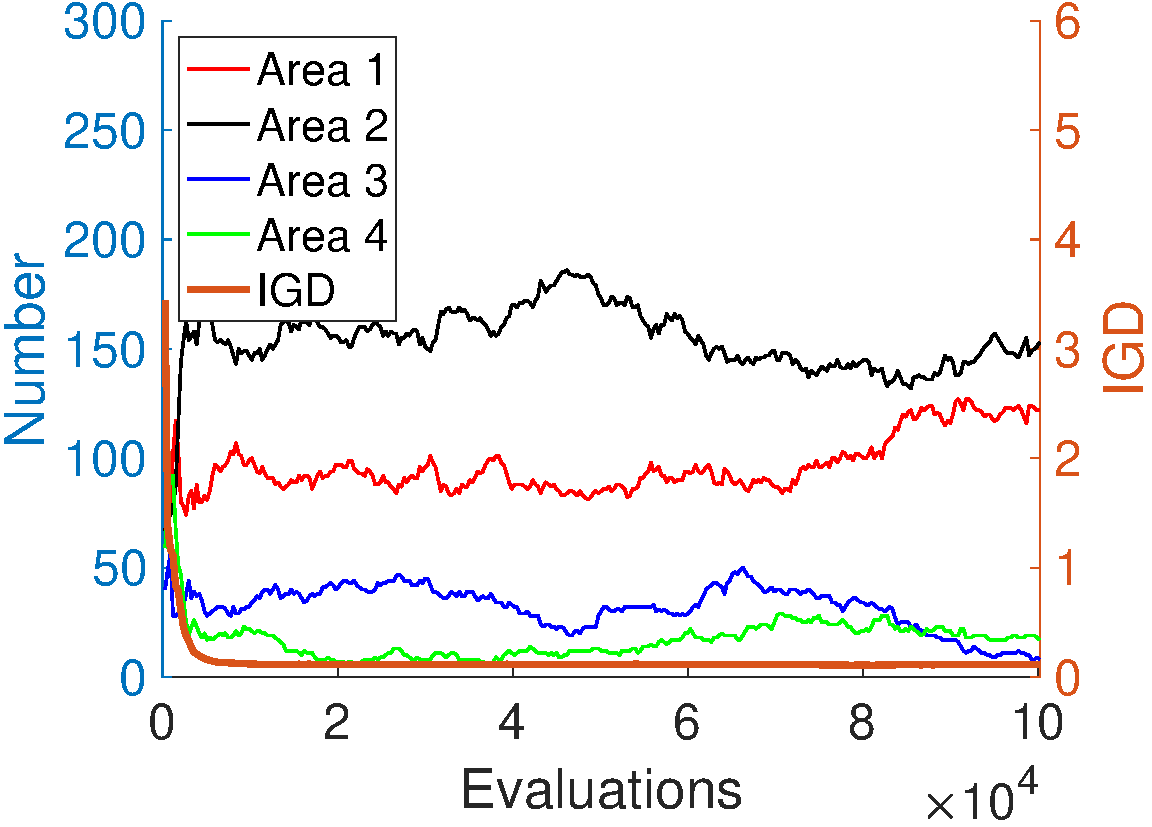
\includegraphics[width=\linewidth]{Section5/dim4/Diversity/SPEA2}
    \caption{SPEA2}
    \end{subfigure}
    \caption{Solution distribution and IGD value of MOEAs on Multi-Polygon test problem with $D=4$.}
    \label{fig: MOEAs Diversity dim=4}
\end{figure}

\begin{figure}[htbp]
    \centering
    \begin{subfigure}[b]{.22\textwidth}
    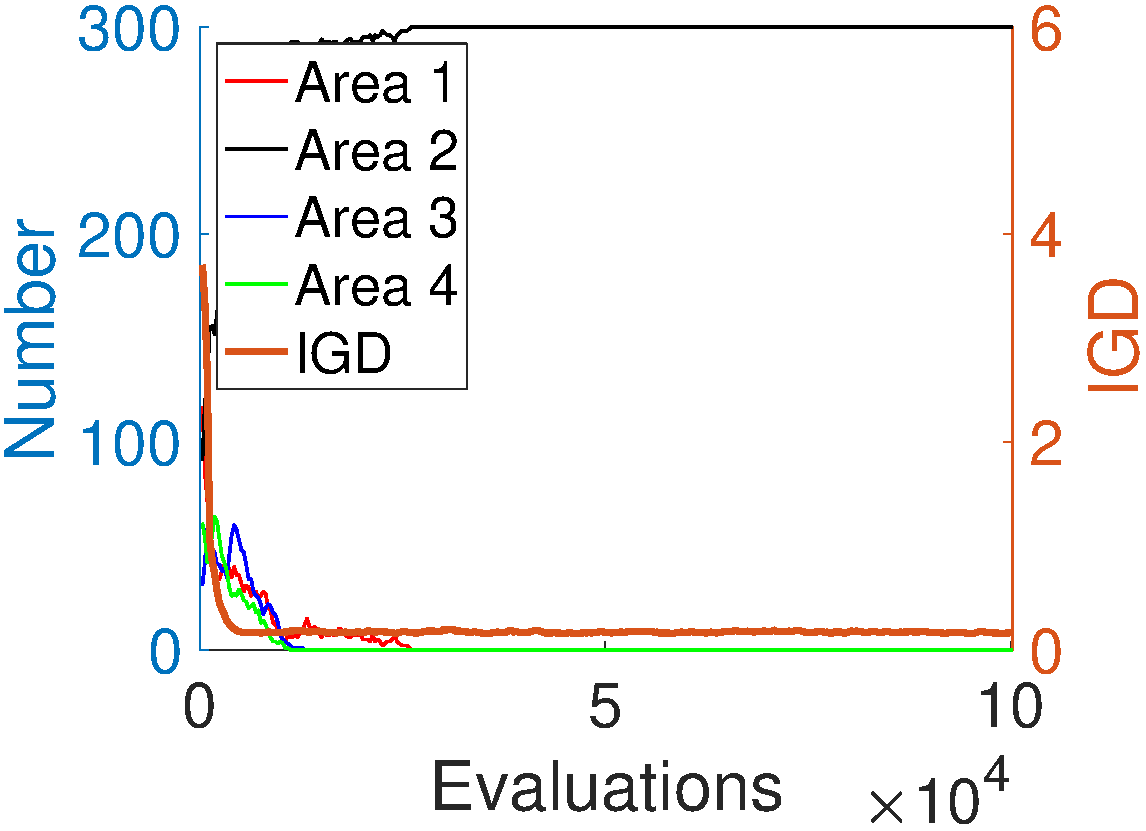
\includegraphics[width=\linewidth]{Section5/dim4/Diversity/DNEA}
    \caption{DNEA}
    \end{subfigure}
    \begin{subfigure}[b]{.22\textwidth}
    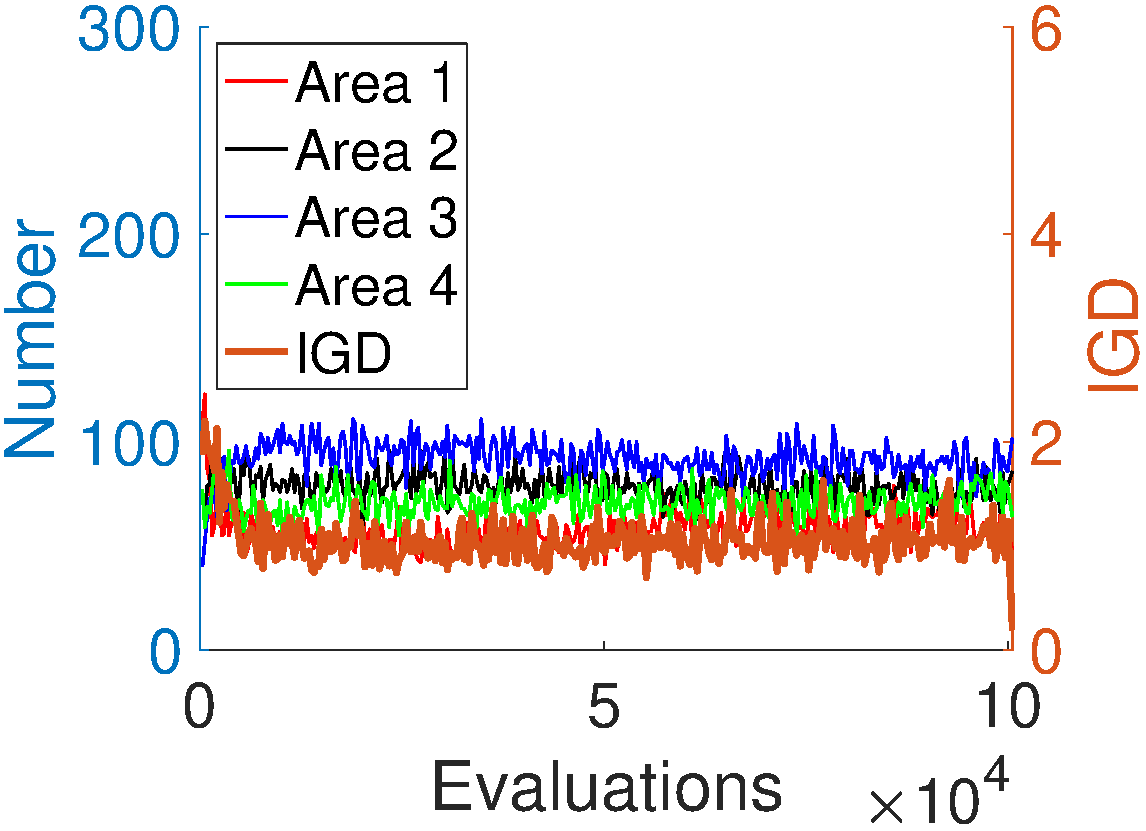
\includegraphics[width=\linewidth]{Section5/dim4/Diversity/MO_Ring_PSO_SCD}
    \caption{MO\_Ring\_PSO\_SCD}
    \end{subfigure}
    
    \begin{subfigure}[b]{.22\textwidth}
    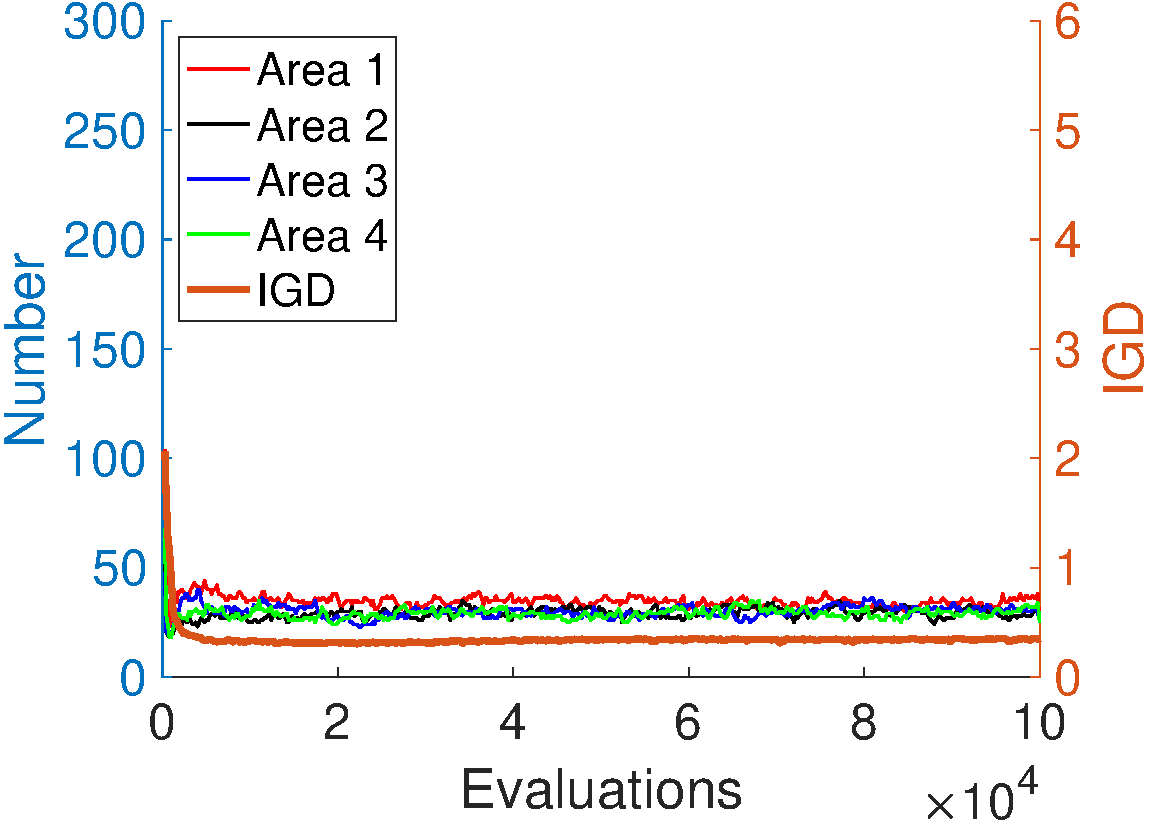
\includegraphics[width=\linewidth]{Section5/dim4/Diversity/MOEADAD}
    \caption{MOEA/D-AD}
    \end{subfigure}
    \begin{subfigure}[b]{.22\textwidth}
    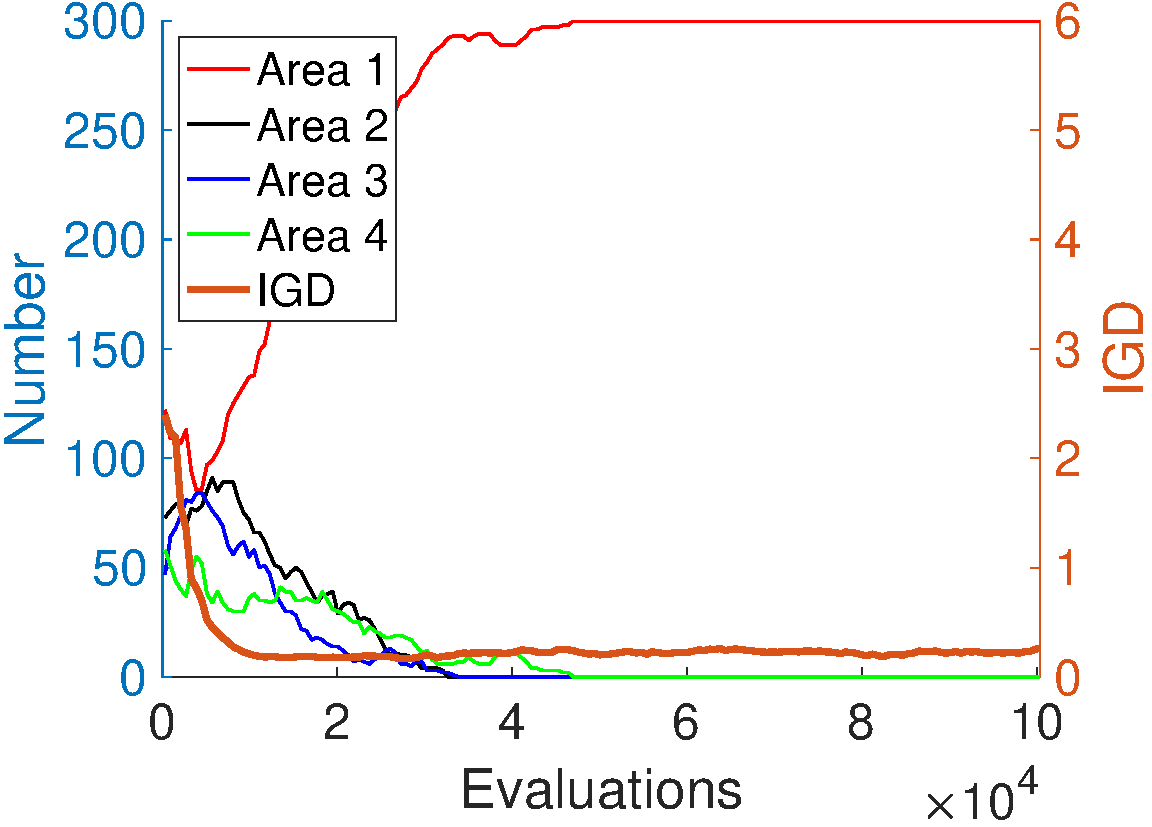
\includegraphics[width=\linewidth]{Section5/dim4/Diversity/OmniOptimizer}
    \caption{Omni-optimizer}
    \end{subfigure}
    \caption{Solution distribution and IGD value of MMEAs on Multi-Polygon test problem with $D=4$.}
    \label{fig: MMEAs Diversity dim=4}
\end{figure}

Due to the page limitation, the simulation results of MOEAs and MMEAs on Multi-Polygons test problem with higher dimensional decision space are not shown here. Instead, we calculate IGD and IGDX values of each algorithm when $D=2, 4, 6, 8, 10, 100$. These two indicators measures the quality of the solution set in objective and decision space respectively. From table \ref{table: IGDX sumup}, it is obvious that MO\_Ring\_PSO\_SCD and MOEA/D-AD have much smaller IGDX values than others which means that the quality of the obtained PS approximation also better than others. These indicator values are consistent with our visualization results.

\begin{table}[htbp]
\begin{tabular}{@{}ccccccc@{}}
\toprule
Algorithms      & D=2                          & D=4                          & D=6                          & D=8                          & D=10                         & D=100                         \\ \midrule
NSGA-II         & 0.14                         & 2.71                         & 4.81                         & 6.67                         & 8.09                         & 28.44                         \\
NSGA-III        & 1.53                         & 3.4                          & 5.2                          & 6.87                         & 8.15                         & 29.56                         \\
MOEA/D-TCH      & 1.17                         & 5.53                         & 6.91                         & 8.13                         & 9.22                         & 31.06                         \\
MOEA/D-PBI      & 1.96                         & 4.96                         & 6.29                         & 7.32                         & 8.26                         & 29.73                         \\
IBEA            & 0.13                         & 1.8                          & 5.03                         & 6.91                         & 7.82                         & 29.52                         \\
SPEA2           & \cellcolor[HTML]{F8FF00}0.11 & 1.84                         & 4.74                         & 6.87                         & 7.85                         & \cellcolor[HTML]{F8FF00}28.45 \\
DNEA            & 0.12                         & 5.13                         & 6.49                         & 7.69                         & 8.73                         & 30.74                         \\
\cellcolor[HTML]{F8FF00}MO\_Ring\_PSO\_SCD & \cellcolor[HTML]{F8FF00}0.11 & 0.33                         & 0.68                         & 1.13                         & 1.9                          & 44.08                         \\
\cellcolor[HTML]{F8FF00}MOEA/D-AD       & 0.19                         & \cellcolor[HTML]{F8FF00}0.28 & \cellcolor[HTML]{F8FF00}0.41 & \cellcolor[HTML]{F8FF00}0.57 & \cellcolor[HTML]{F8FF00}0.82 & 32.96                         \\
Omni-optimizer  & 0.16                         & 5.08                         & 6.47                         & 7.83                         & 9.02                         & 30.62                         \\ \bottomrule
\end{tabular}
\caption{IGDX values}
\label{table: IGDX sumup}
\end{table}

 However, from the perspective of objective space, the situation will be different. As shown in table \ref{table: IGD sumup}, the performance of MMEAs is worse than MOEAs especially when D is large. Indicator based algorithms IBEA and SPEA2 obtain best PF approximation. From here we can roughly assume that maintaining the diversity of the decision space is not without cost. The seach ability of MMEAs in objective space is lower than general MOEAs.

\begin{table}[htbp]
\begin{tabular}{@{}ccccccc@{}}
\toprule
Algorithms      & D=2                          & D=4                          & D=6                          & D=8                          & D=10                        & D=100                        \\ \midrule
NSGA-II         & 0.1                          & 0.17                         & 0.25                         & 0.33                         & 0.41                        & 3.01                         \\
NSGA-III        & 0.14                         & 0.21                         & 0.28                         & 0.33                         & 0.39                        & 3.95                         \\
MOEA/D-TCH      & 0.26                         & 0.41                         & 0.64                         & 0.93                         & 1.2                         & 6.76                         \\
MOEA/D-PBI      & 0.11                         & 0.16                         & 0.2                          & 0.25                         & 0.3                         & 4.22                         \\
\cellcolor[HTML]{F8FF00}IBEA            & 0.09                         & 0.13                         & \cellcolor[HTML]{F8FF00}0.15 & \cellcolor[HTML]{F8FF00}0.17 & \cellcolor[HTML]{F8FF00}0.2 & 3.9                          \\
\cellcolor[HTML]{F8FF00}SPEA2           & \cellcolor[HTML]{F8FF00}0.07 & \cellcolor[HTML]{F8FF00}0.12 & 0.16                         & 0.2                          & 0.24                        & \cellcolor[HTML]{F8FF00}2.73 \\
DNEA            & 0.08                         & 0.17                         & 0.31                         & 0.5                          & 0.67                        & 5.91                         \\
MO\_Ring\_PSO\_SCD & 0.1                          & 0.19                         & 0.4                          & 0.72                         & 1.12                        & 57.46                        \\
MOEA/D-AD       & 0.27                         & 0.36                         & 0.47                         & 0.58                         & 0.72                        & 12.97                        \\
Omni-optimizer  & 0.09                         & 0.22                         & 0.45                         & 0.7                          & 0.95                        & 5.54                         \\ \bottomrule
\end{tabular}
\caption{IGD values}
\label{table: IGD sumup}
\end{table}
\section{Concluding Remarks}
This article mainly made two contributions. Firstly, we addressed in detail the difficulties in solving MMOPs, which has not been carefully analyzed before. On the one hand, we pointed out that the selection, mutation and crossover process in classical MOEAs will cause problem for handling MMOPs. On the other hand, genetic drift concept is introduced to explain the the phenomenon that the equivalent solution disappears during the evolutionary process by treating equivalent solutions as alleles. Our analysis may help to develop special mechanisms to counter the effect of genetic drift. 

Secondly, a series of computational experiments is conducted to examine the performance of MOEAs and MMEAs on Multi-Polygon test problem. The experimental results shows that the adaptability of DNEA and Omni-optimizer is poor. Another two MMEAs MO\_Ring\_PSO\_SCD and MOEA/D-AD can obtain best PS approximation compared to other candidate algorithms. We also pointed that on Multi-Polygons test problem, the search ability of MMEAs in decision space is lower than classical MOEAs. In future research, more experiments are needed to reveal the effect of diversity maintenance mechanisms in decision space to the quality of search ability in objective space.

\section*{Acknowledgment}
This work was supported by the Program for Guang- dong Introducing Innovative and Enterpreneurial Teams (Grant No. 2017ZT07X386), Shenzhen Peacock Plan (Grant No. KQTD2016112514355531), the Science and Technol- ogy Innovation Committee Foundation of Shenzhen (Grant No. ZDSYS201703031748284), the Program for Univer- sity Key Laboratory of Guangdong Province (Grant No. 2017KSYS008), and National Natural Science Foundation of China (Grant No. 61876075).
\bibliographystyle{ieeetr}
\bibliography{References.bib}

\end{document}
